\documentclass[10pt,a4paper,titlepage]{article}
\usepackage[T1]{fontenc}
\usepackage[utf8]{inputenc}
\usepackage[french]{babel}
\usepackage{hyperref}
\usepackage[pdftex]{graphicx}
\usepackage[a4paper,left=2cm,right=2cm,top=2cm,bottom=2cm]{geometry} % A personaliser
\usepackage{libertine}
\usepackage{dirtree}
% Custom colors
\usepackage{color}
%\usepackage[hashEnumerators,smartEllipses]{markdown}
\usepackage[most]{tcolorbox}
\usepackage{tikz,lipsum,lmodern}
\usepackage{listings}
\usepackage{graphicx}
\usepackage[]{caption}
\usepackage{siunitx}
\usepackage{mathtools}
\DeclarePairedDelimiter\abs{\lvert}{\rvert}%
\DeclarePairedDelimiter\norm{\lVert}{\rVert}%
% Swap the definition of \abs* and \norm*, so that \abs
% and \norm resizes the size of the brackets, and the 
% starred version does not.
\makeatletter
\let\oldabs\abs
\def\abs{\@ifstar{\oldabs}{\oldabs*}}
\let\oldnorm\norm
\def\norm{\@ifstar{\oldnorm}{\oldnorm*}}

% Custom highlight rules for Python
\definecolor{paramColor}{rgb}{0.2,0.2,0.9}
\definecolor{dataColor}{rgb}{0.2,0.8,0.8}
\definecolor{workColor}{rgb}{0.7,0.2,0.8}
\definecolor{outputColor}{rgb}{0.4,0,0.5}
\definecolor{deepblue}{rgb}{0,0,0.5}
\definecolor{deepred}{rgb}{0.6,0,0}
\definecolor{deepgreen}{rgb}{0,0.5,0}
\definecolor{darkgrey}{rgb}{0.6,0.6,0.6}
\definecolor{lightgrey}{rgb}{0.8,0.8,0.8}
\definecolor{deeporange}{rgb}{0.8,0.5,0.5}
\lstset{language=Python,
    basicstyle=\ttfamily\small\color{black},
    keywordstyle=\color{deepblue},
    commentstyle=\color{darkgrey},
    stringstyle=\color{deepgreen},
    numberstyle=\color{deeporange},
    showstringspaces=false,
    identifierstyle=\color{deepred},
    tabsize=4
}
\lstset{literate=*
    {0}{{{\color{deeporange}0}}}1
    {1}{{{\color{deeporange}1}}}1
    {2}{{{\color{deeporange}2}}}1
    {3}{{{\color{deeporange}3}}}1
    {4}{{{\color{deeporange}4}}}1
    {5}{{{\color{deeporange}5}}}1
    {6}{{{\color{deeporange}6}}}1
    {7}{{{\color{deeporange}7}}}1
    {8}{{{\color{deeporange}8}}}1
    {9}{{{\color{deeporange}9}}}1
}

%\usepackage[
%backend=biber,        % compilateur par défaut pour biblatex
%sorting=nyt,          % trier par nom, année, titre
%citestyle=authoryear, % style de citation auteur-année
%bibstyle=alphabetic,  % style de bibliographie alphabétique
%]{biblatex}
% quand tu auras créé ton fichier bib
% \addbibresource{ton-fichier-biblio.bib}
\usepackage{biblatex}
\addbibresource{../rapport-AB.bib}
\addbibresource{../bibliography.bib}


% Pour t'aider à créer et citer la biblio dans le texte, tu peux aller à cette page:
% -> https://bu.univ-amu.libguides.com/c.php?g=511707&p=3496584

\setlength{\parindent}{0.4cm}
\setlength{\parskip}{1ex plus 0.5ex minus 0.2ex}
\newcommand{\hsp}{\hspace{20pt}}
\newcommand{\HRule}{\rule{\linewidth}{0.5mm}}
\newtcolorbox{processEnv}[2][]{width=\linewidth, colframe=white!97!black, colback=white!95!black, boxrule=5pt, enhanced, breakable, attach boxed title to top center={yshift=-4mm}, title={#2}, colbacktitle=white!55!black}
\newtcolorbox{codeEnv}[2][]{
    width=\linewidth, colframe=white!85!black, colback=white!95!black, boxrule=2pt, enhanced, breakable, attach boxed title to top center={yshift=-4mm}, coltitle = white!20!black, title={#2}, colbacktitle=white!75!black}

\def\siecle#1{\textsc{\romannumeral #1}\textsuperscript{e}~siècle}

\begin{document}

  \begin{titlepage}
      \begin{sffamily}
          \begin{center}

              % Upper part of the page. The '~' is needed because \\
              % only works if a paragraph has started.
              %\includegraphics[scale=0.04]{img1.JPG}~\\[1.5cm]

              \textsc{\LARGE ENS de Lyon, Université Lyon1}\\[2cm]

              \textsc{\Large Rapport de Master 2}\\[1.5cm]

              % Title
              \HRule \\[0.4cm]
              { \huge \bfseries Mise en place d’un modèle numérique hydrodynamique de l’anse du Cul-de-Loup (Normandie, France) Opérateur expédition produits finis\\ [0.4cm] }

              \HRule \\[2cm]
              %\includegraphics[scale=0.2]{img2.JPG}
              %\\[2cm]

              % Author and supervisor
              \begin{minipage}{0.4\textwidth}
                  \begin{flushleft} \large
                      \emph{Auteure :} Mme \textsc{A. BONVALET}\\
                  \end{flushleft}
              \end{minipage}
              \begin{minipage}{0.4\textwidth}
                  \begin{flushright} \large
                      \emph{Tuteur :} M. \textsc{E. POIZOT}\\
                  \end{flushright}
              \end{minipage}

              \vfill

              % Bottom of the page
              {\large Janvier 2025 — Juin 2025}

          \end{center}
      \end{sffamily}
  \end{titlepage}

\tableofcontents
\newpage

\section{INTRODUCTION}
\label{sec:introduction}

%
%A faire presque à la fin, mais les grandes idées seront:
%\begin{itemize}
%    \item changement climatique, pression anthropique: besoin de gérer l'espace côtier
%    \item modèles numériques, outils pour réaliser divers scénarios pour une bonne gestion
%    \item anse du cul-de-loup (ADCL): un bon exemple de nécessité de gestion raisonnée
%    \item utilisation du code de calcul CROCO pour réaliser un modèle numériques de ADCL
%\end{itemize}
%


A l'interface entre les terres et les mers, les zones côtières ont toujours été attractives pour l'Homme, qu'il s'agisse d'y développer des activités économiques ou tout simplement pour y habiter. L’essor industriel des deux cent dernières années a accru la pression anthropique sur ces zones, avec un développement urbain et industriel croissant\footnote{Actuellement, plus de 20\% de la population mondiale vit à moins de 30 km des côtes \cite{senat2015}.}. Depuis environ soixante dix ans, l'accélération quasi exponentielle de ces activités a engendré d'un côté une disparition progressive des espaces naturels côtiers et de l'autre un dérèglement du climat avec une montée régulière du niveau moyen des océans \cite{ipcc2021}. Ce double effet fait aujourd'hui courir de grands risques aux zones côtières.

En France, l'activité de culture d'huître est une source importante de revenus pour certaines régions (Haut de France, Normandie, Bretagne, Pays de la Loire, Charente-Maritime, Aquitaine). En Normandie, le département de la Manche, avec ses 670 km de côtes, produit plus de \num{15000} tonnes d'huîtres par an. Depuis le \siecle{18}, le Cotentin abrite sur ses côtes des activités conchylicoles \cite{Kopp2000}. Tout d'abord artisanale, cette culture consistait en un reparquage d'huître plates locales. À partir du \siecle{20} (début des années 60), la conchyliculture normande connaît une phase d'expansion importante et devient industrielle. De nouvelles zones côtières sont investies pour implanter les concessions ostréicoles et des aménagements sont réalisés pour en faciliter l'implantation.
Avec certains de ses secteurs encore sauvages, les côtes Normandes ont aussi un attrait touristique de villégiature ainsi qu'historique\footnote{Notamment en relation avec les évènements de la seconde guerre mondiale et le débarquement du 6 juin 1944.}.  C'est aussi un secteur d'activité important pour de nombreuses communes côtières de cette région, antagoniste d'activités industrielles telles que la conchyliculture.

L'anse du Cul-de-Loup (Normandie, Manche, France, Fig. \ref{fig:carte-adcl}) est un exemple typique de l'évolution au cours du temps des côtes du littoral français (Fig. \ref{fig:historique-adcl}). Avec la prise de conscience de la nécessaire préservation des milieux naturels, de nombreuses zones côtières telles que l'anse du Cul-de-Loup ont vu des mesures de sauvegarde mises en place, via la création de sites Natura 2000, les classements ZNIEFF\footnote{Zones naturelles d’Intérêt Écologique, Faunistique et Floristique.} (1 et 2) ou encore les directives habitat faune et flore. Malgré ces initiatives de préservation d'un milieu naturel fragile, l'anse du Cul-de-Loup connaît une dégradation de son environnement, avec une disparition progressive de certaine communauté d'algues protégées (la Zostère et Spatine marine), ainsi qu'un envasement de plus en plus important au détriment de la couverture sableuse originale.

L'état français via ses agences dédiées (Agence de l'Eau, IFREMER, etc.), mais aussi les entités régionales (Région Normandie) et locale (Département de la Manche), financent des travaux et projets dans une optique d'amélioration de la gestion de l'espace de l'anse du Cul-de-Loup. Ainsi, l'Agence de l'Eau Seine-Normandie (AESN) a financé le programme scientifique "\textit{Projet de Territoire : Anse du Cul-de-Loup}" (ProTeC) de 2022 à 2024, dans l'objectif de dresser un état des lieux environnemental. Ce travail a permis de connaître de manière précise, la nature des cortèges sédimentaires de surface de l'anse, ainsi que sa dynamique de mise en place. Les courants étant le moteur principal des mouvements de sédiment, des mesures de vitesses et directions de la masse d'eau ont été acquises, cumulant trois mois de mesures en deux points à l'entrée de l'anse du Cul-de-Loup. Bien que cet effort de mesure soit déjà important, il n'est pas suffisant pour aborder l'hydrodynamique à l'échelle de l'anse toute entière.

Seuls les modèles numériques hydrodynamiques peuvent offrir la possibilité d'avoir une telle information spatialement répartie à des coûts acceptables. Ce type d'outil offre la possibilité d'avoir, outre le spatial, une approche temporelle, soit en rejouant des conditions hydrodynamiques passées (utiles pour la validation du modèle), soit au contraire en simulant des conditions futures (utiles pour la gestion de l'espace). Aux échelles spatiales et temporelles d'intérêts, ce sont les modèles de type \textit{Reynolds Average Navier-Stokes} (RANS) les mieux adaptés pour modéliser/simuler les écoulements fluides.
Le travail qui m'a été demandé dans le cadre de mon stage de seconde année de Master, est de mettre en place un modèle numérique hydrodynamique de l'anse du Cul-de-Loup à l'aide du code de calcul \textit{Coastal and Regional Ocean COmmunity model} (CROCO) (section \ref{sub:croco}). Dans la section \ref{sec:adcl}, je décris brièvement la zone d'étude de l'anse du Cul-de-Loup dans laquelle ont été acquise les données de mesures des courants (section \ref{sub:protec}). Les résultats de la mise en place du modèle numériques sont présentés dans la section \ref{sec:resultats} et la comparaison avec les mesures de terrains est située en section \ref{sec:discussion}. Dans la conclusion (section \ref{sec:conclusion}), je dresse un bilan du travail réalisé et donne des perspectives de travaux complémentaires.

\newpage

\section{ZONE D'ÉTUDE}
\label{sec:adcl}


D'une superficie avoisinant les 370 ha, l'anse du Cul-de-Loup n'est ouverte que dans sa partie sud sur la baie de Seine. La fermeture complète de l'anse, à l'est, a été réalisée au cours du \siecle{17} par la construction d'une route-digue qui rejoint le continent depuis St-Vaast-la-Hougue à l'ex île de la Hougue (Fig. \ref{fig:carte-adcl}). L'ensemble de l'anse découvre plus ou moins en fonction des coefficients de marée (marée semi-diurne), avec un marnage d'environ 5 m en marée de vive eau. Le zéro hydrographique est situé juste à l'entrée de l'anse parallèlement à la ligne côtière. L'altitude maximum dans l'anse ne dépasse pas 3 m au dessus du zéro hydrographique.

\begin{figure}[!h]
    \centering
    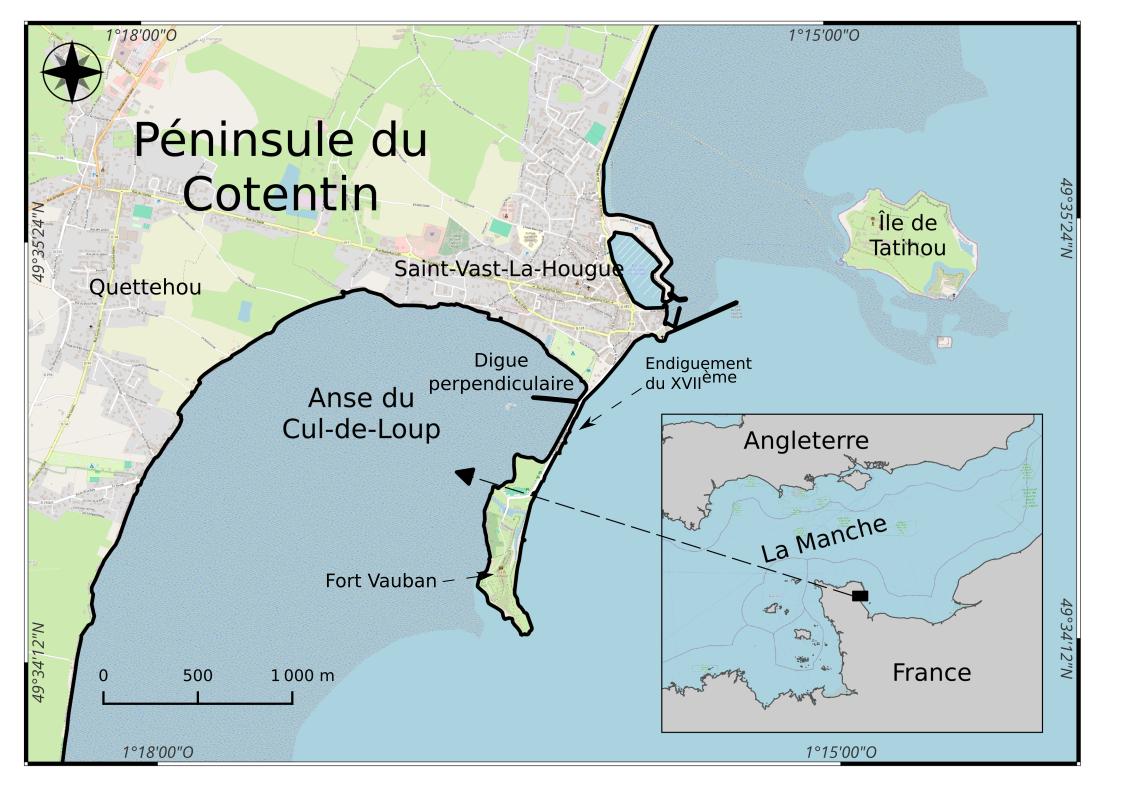
\includegraphics[width=0.8\linewidth]{../images/carte-ADCL}
    \caption[Anse du Cul-de-Loup.]{L'anse du Cul-de-Loup.}
    \label{fig:carte-adcl}
\end{figure}

Le vent est régulièrement présent sur la zone du Cul-de-Loup, avec une moyenne de 18-19 km/h l'été majoritairement de secteur ouest et de 25-30 km/h en période hivernale avec un partage plus homogène des directions. L'agitation de surface dans l'anse est majoritairement de type mer du vent, due au frottement par le vent à la surface de l'eau.

L'orientation de l'anse du Cul-de-Loup la protège des houles les plus fréquentes en Baie de Seine, qui sont de secteurs nord-ouest à nord-est essentiellement. Les houles de secteur est et sud-est sont les seules à éventuellement pouvoir pénétrer dans l'anse, mais elles sont à la fois plus rares et de faible énergie. Ces dernières sont rapidement dissipées par la présence des structures ostréicoles et pénètrent donc peu à l'intérieure de l'anse. A l'est au niveau de la bordure interne de l'Île de la Hougue, certaines houles peuvent néanmoins diffractées et être canalisées le long de l'île avec une énergie significative.

\begin{figure}[!h]
    \centering
    \includegraphics[width=0.8\linewidth]{../images/historique}
    \caption[Évolution de l'anse du Cul-de-Loup]{En bas à gauche, image aérienne de 1942, l'anse du Cul-de-Loup ne contient aucun parc ostréicole. En bas à droite, image aérienne de 1965, l'anse du Cul-de-Loup commence à être aménagée dans sa partie nord. En haut à gauche et à droite, respectivement la morpho-bathymétrie  et une image aérienne actuelle de l'anse du Cul-de-Loup montrant de nombreuses concessions ostréicoles.}
    \label{fig:historique-adcl}
\end{figure}



\newpage

\section{MATÉRIELS ET MÉTHODES}
\label{sec:materiel_methodes}
\subsection{Le code de calcul CROCO}
\label{sub:croco}

\subsubsection{Présentation générale}
\label{subsub:presentation_generale}
%Mettre les principes généraux de CROCO (origine, type de modèle, etc...)
Le modèle CROCO (\textit{Coastal and Regional Ocean COmmunity model}) est une évolution du code ROMS\_AGRIF (\textit{Regional Oceanic Modeling System with mesh refinement}).
Le code ROMS\_AGRIF a été développé jusqu'en 2014 par l'IRD (\textit{Institut de Recherche pour le Développement}) et l'INRIA (\textit{Institut National de Recherche en Informatique et en Automatique}) qui ont participé au développement du code CROCO avec
l'UPS (?), 
l'IFREMER (\textit{Institut Français de Recherche pour l'Exploitation de la Mer}), 
le SHOM (\textit{Service hydrographique et océanographique de la Marine}), 
le CNRS (\textit{Centre National de la Recherche Scientifique})
et les participants de ROMS comme et principalement 
l'UCLA (\textit{University of California, Los Angeles}) 
et la DGEO (\textit{Departamento de Geofísica Universidad de Concepción}). 
Le code et la documentation de ROMS\_AGRIF ont progressivement été modifiés pour devenir le modèle communautaire CROCO.

Ce modèle permet désormais de réaliser des modélisations sur des grilles dont la résolution peut être kilométrique (modèle régional) à métrique (modèle côtier).

CROCO permet d'activer la parallélisation des calculs effectués lors de la modélisation. Ainsi, pour certaines configurations, il est possible de modéliser des temporalités de l'ordre de l'année pour une coût de calcul abordable. (ex .)

Le système d'équations utilisées par le modèle est flexible, il permet de choisir la méthode de résolution physico-chimique voulue et adaptée à la configuration.
Les systèmes d'équations sont progressivement vérifiées par la communauté avec la mise en place de cas test dont la physique est simple. % dont on sait quel résultat est attendu pour quel système d'équation.

Les forçages physico-chimiques initiaux et aux limites sont la source des mouvements dans la masse d'eau.
Ils sont intégralement choisis par l'utilisateur·ice de CROCO.
Ces forçages peuvent contenir une large variété de données spatiales et temporelles.
On relèvera notamment la possibilité d'indiquer la valeur des températures, des salinités, des hauteur d'eau relativement au niveau marins de référence, des vitesses de courant et des conditions atmosphériques à proximité de la surface.
Les données des forçages sont rassemblées au sein de plusieurs fichiers.
Ces dernières sont regroupées dans cinq principaux fichiers comme listé ci-dessous:

\begin{itemize}
    \item le contexte physique du domaine modélisé (bathymétrie, limite côte-océan, etc.);
    \item les phénomènes physiques externes à la masse d'eau qui forcent son déplacement :
    \begin{itemize}
        \item[.] la marée (amplitude et vitesse de d'placement de l'onde de marée),
        \item[.] les conditions atmosphériques (vent, pluie, etc.),
    \end{itemize}
    \item les conditions physico-chimiques internes à la masse d'eau aux limites durant la période modélisées (température salinité, etc.),
    \item les mêmes conditions physico-chimiques dans l'ensemble de la zone modélisée au départ du modèle.
\end{itemize}
Ces fichiers doivent respecter une structure et une nomenclature particulière afin d'être utilisables par le code CROCO.
Un schéma global de la mise en place du modèle est présenté en Figure \ref{fig:workflow_simple}
\begin{figure}[h!]
    \centering
    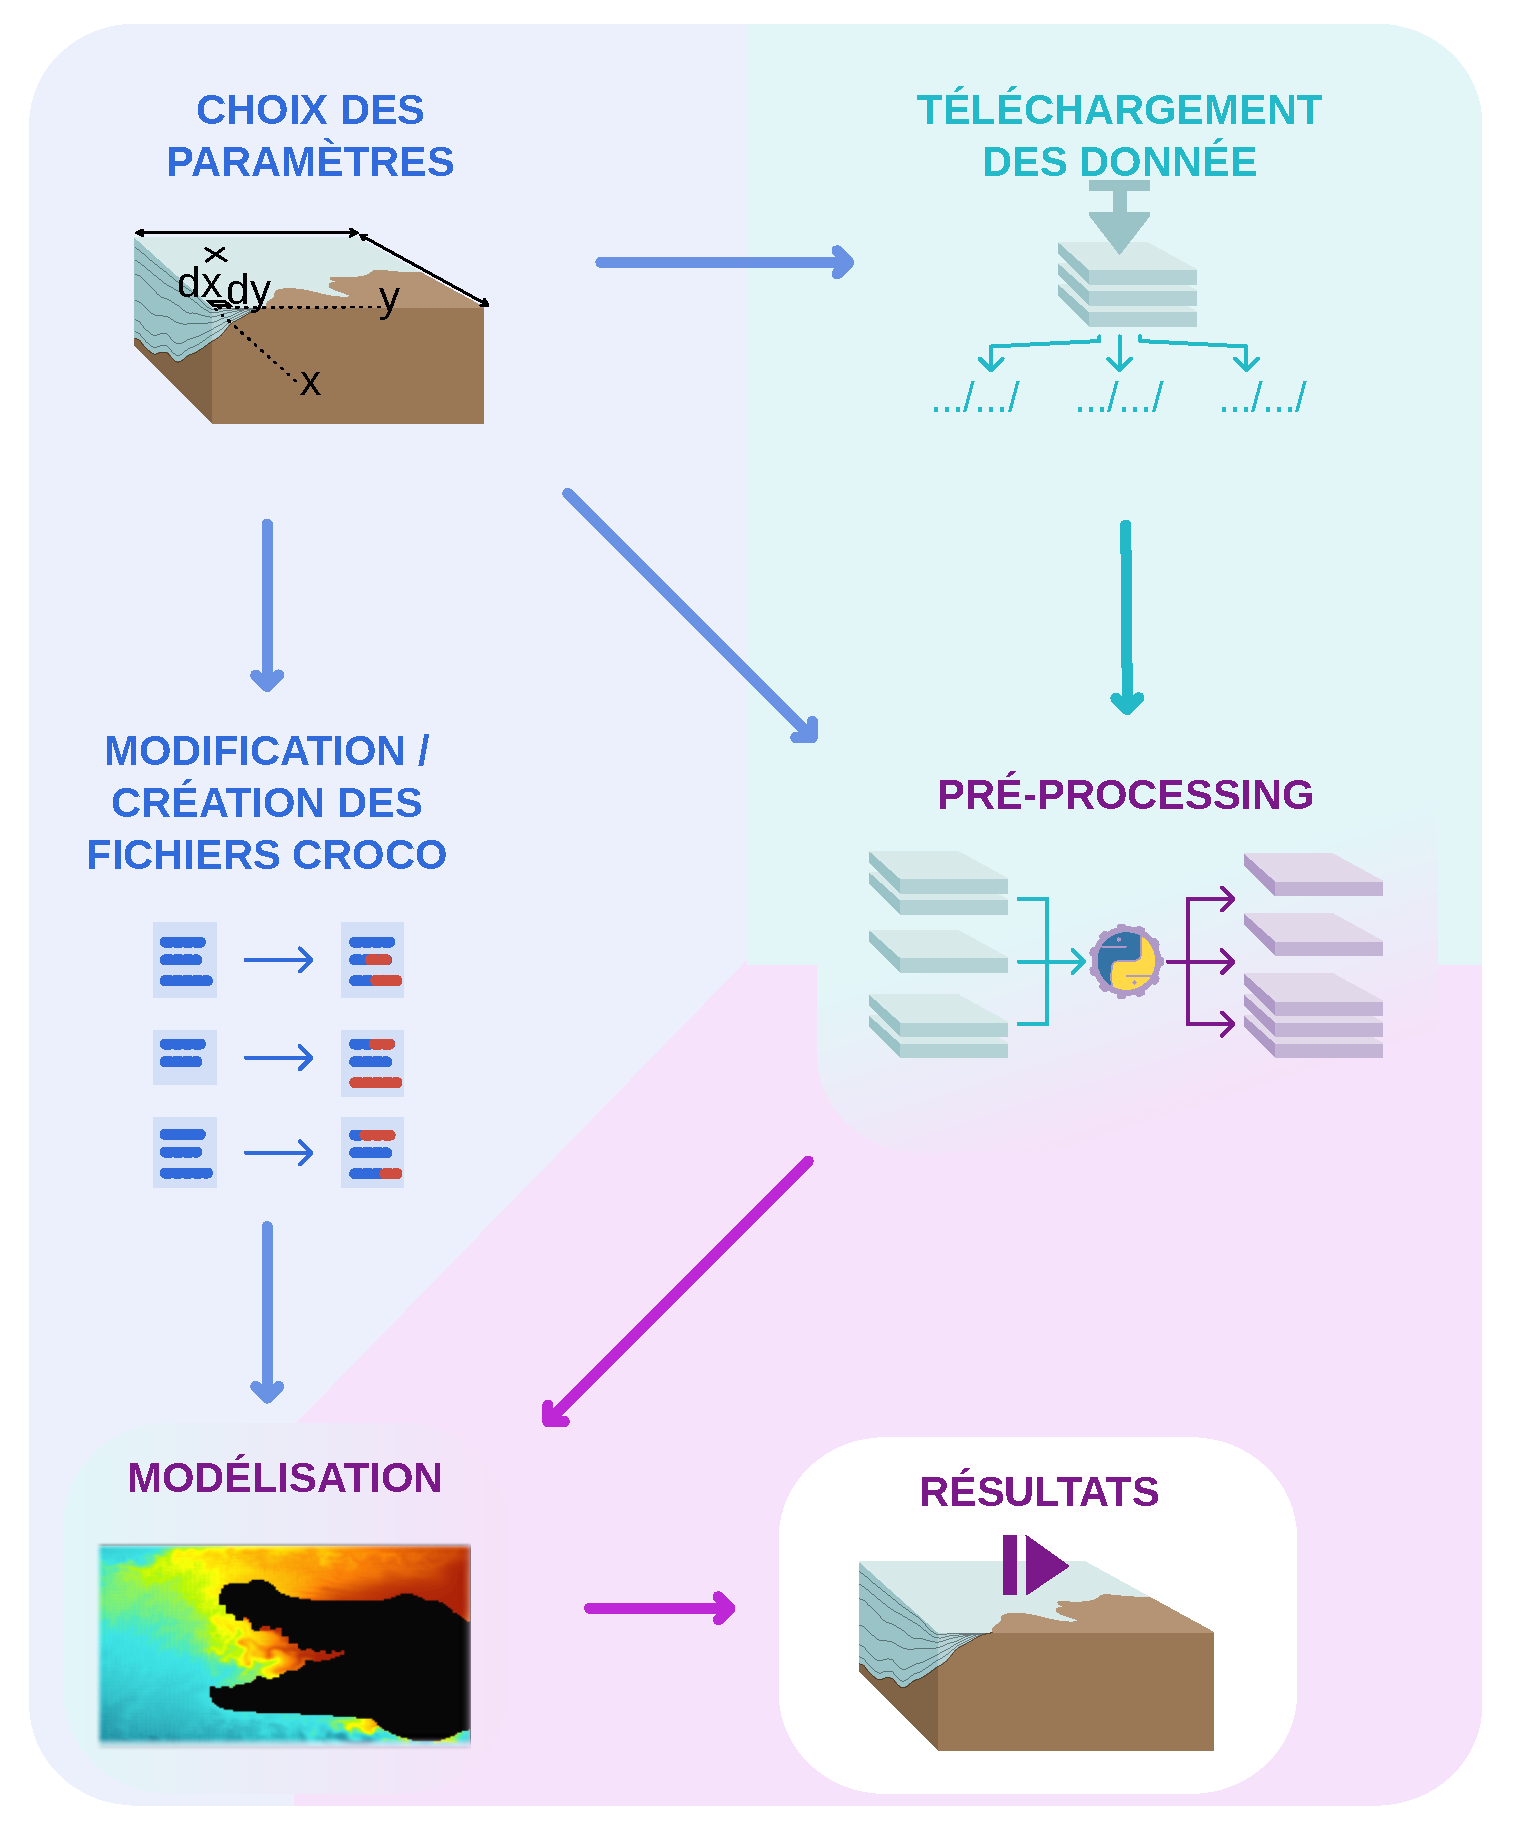
\includegraphics[scale=0.35]{../images/workflow/mise_en_place_generale_croco.pdf}
    \caption{
        \textbf{Mise en place du modèle CROCO avec une gille simple.}
        \\Les flèches larges correspondent à l'utilisation d'un ou plusieurs fichiers pour la génération d'un ou de plusieurs autres.
        L'action nécessaire est décrite en bout de flèche.
        Lorsque les flèches ne se suivent pas, les étapes peuvent être effectuées en parallèle.
        Toutefois la mise en place de la modélisation est plus intuitive en suivant l'ordre : {\color{paramColor}choix des paramètres}, {\color{dataColor} téléchargement des données}, {\color{workColor} pré-traitement}, {\color{paramColor} modification des fichiers CROCO}, {\color{workColor} modélisation (compilation et exécution de CROCO)}.
    }
    \label{fig:workflow_simple}
\end{figure}

Enfin, en même temps que le développement du modèle, des outils communautaires de pré- et de post- traitement adaptés au fonctionnement de CROCO ont été développés.
Ces outils ont d'abord été écrits en Matlab sous le nom de CROCO\_tools mais, pour mieux correspondre à la dynamique open-source de CROCO, de nouveaux outils, les CROCO\_Pytools, sont en cours de développement en Python.

%Afin de simplifier le travail de pré-traitement, la communauté a développé des outils numériques de lecture, calcul et écriture de données.
%Ces codes de pré-traitement utilisent au choix des scripts Matlab (ces outils sont appelés croco\_tools) ou des scripts Python (ces outils sont appelés croco\_pytools).
%L'utilisation dans le cadre du stage de ces outils est décrite dans la partie suivante.

\subsubsection{Les variables modélisées}
\label{subsub:variables_modelisees}
Le modèle CROCO permet la propagation de variables physico-chimiques qui ont un effet rétroactifs sur leur propre propagation ou-et sur la propagation d'autres variables.
Selon leur type, les paramètres physico-chimiques sont définis à différentes localisations relativement au maillage.
La table \ref{structure_maille horizontale} % https://croco-ocean.gitlabpages.inria.fr/croco_doc/model/model.grid.html -> Grid staggering
illustre les trois positions, appelées ici U, V et H, que peuvent avoir ces variables.

\begin{table}
    \centering
    \begin{tabular}{ c c c }
        \multicolumn{1}{r}{·--} & $V_{i,{\color{red}j+1}}$ & \multicolumn{1}{l}{--·} \\ 
        | & & | \\
        | & & | \\
        $U_{i,j}$ & $H_{i,j}$ & $U_{{\color{red}i+1},j}$ \\  
        | & & | \\
        | & & | \\
        \multicolumn{1}{r}{·--} & \textbf{$V_{i,j}$} & \multicolumn{1}{l}{--·}
    \end{tabular}
    \caption{Représentation d'une maille $i,j$ horizontale de la grille CROCO.
        Les points sont des nœuds et les tirets sont les cotés de la maille.
        La position à laquelle est calculé chaque type paramètre de la maille est représentée par $U_{i,j}$, $V_{i,j}$ et $H_{i,j}$ leur première lettre correspondent au type des paramètres quelles représentent.
        L'existence des paramètres $V_{i,j+1}$ et $U_{i+1,j}$ suppose que la maille $i,j$ ne se situe pas à l'extrémité d'une ligne ou d'une colonne de la grille CROCO.
    }
    \label{structure_maille horizontale}
\end{table}

Une importante part des variables sont localisées en \textbf{position centrale H} au maillage.
Ces variables sont :
\begin{itemize}
    \item la hauteur de la colonne d'eau relativement au niveau marin moyen (à vérifier),
    \item la température de l'eau,
    \item la salinité de d'eau,
    \item l'ensemble des paramètres décrivant les ondes de marrée (phase et amplitude de la hauteur d'eau ainsi que celles des deux composantes des courants induits),
    \item l'ensemble des paramètres atmosphériques à l'exception du vent (précipitation, température de l'air, vitesse absolue et direction du vent à $10m$ au dessus de la surface de l'eau, etc.).
\end{itemize}
Les paramètres localisés à la \textbf{position U} du maillage sont:
\begin{itemize}
    \item la composante Est-Ouest de la vitesse de déplacement de l'eau,
    \item la contrainte à la surface de l'eau causée par la composante Est-Ouest du vent,
    \item la composante Est-Ouest de la vitesse de déplacement de l'air à $10m$.
\end{itemize}
Enfin, les paramètres localisés à la \textbf{position V} du maillage sont:
\begin{itemize}
    \item la composante Nord-Sud de la vitesse de déplacement de l'eau,
    \item la contrainte à la surface de l'eau causée par la composante Nord-Sud du vent,
    \item la composante Nord-Sud de la vitesse de déplacement de l'air à $10m$.
\end{itemize}

Pour tous les paramètre, ils ne sont par exprimés et pas pris en compte aux points indiqués comme émergés par la grille.
Certains de ces paramètres sont exprimés sur l'intégralité du maillage horizontal et vertical.
D'autres ne le sont qu'aux limites de la grille, c'est à dire sur tout le tour de cette dernière.
D'autres encore sont exprimés sur toutes l'étendue horizontale de la grille mais uniquement en surface ou au fond.

L'ensemble de ces paramètres définissent les forçages physico-chimiques imposés au modèle.
Ils sont regroupés dans plusieurs fichiers selon la manière dont ils influent sur le modèle.

La première catégorie contient les forçages qui définissent les conditions initiales.
Le fichier correspondant contient donc les données de hauteur d'eau, de courant, de température et de salinité sur l'ensemble de la grille à l'initialisation du modèle.

La seconde catégorie contient les forçages qui définissent les conditions aux bords latéraux de la grille.
Le fichier correspondant contient donc les données de hauteur d'eau, de courant, de température et de salinité aux bords de la grille durant le temps de la modélisation.

La troisième catégorie contient les forçages de marrée.
%Ces derniers remplacent les données de hauteur d'eau et éventuellement de courant des conditions aux bordures. 
Le fichier correspondant contient donc, pour $n$ harmoniques de marrée, les amplitudes et les phases des hauteurs d'eau et éventuellement les deux composantes horizontales de la vitesse de déplacement de l'onde de marrée.

La quatrième catégorie contient forçages atmosphériques.
Ils concernent la surface de l'eau et l'air qui la surplombe pour chaque maille de la grille CROCO.
Le fichier correspondant contient donc notamment l'humidité, la température, la pression de l'air au dessus de la surface de l'eau, la vitesse du vent à $10m$ au dessus de la surface, des paramètres sur les contraintes de surfaces imposés par le vent et les radiations solaires reçues par la masse d'eau pour les courtes et longues longueurs d'ondes.

\subsubsection{Physique du modèle}
\label{subsub:pysique_modele}
Lors de sa compilation, CROCO utilise le fichier \textit{cppdef.h}, l'un des quatre fichiers dont le contenu est modifié par l'utilisateur·ice, pour déterminer quelles équations physiques doivent être résolues par le modèle.
Ces fichiers sont représentés en bleu en Figure \ref{fig:workflow_simple}.

Pour les modélisations effectuées dans le cadre du stage, le contenu du fichier a été modifié pour que les équations résolues correspondent à un schéma d'advection de cinquième ordre \ref{WENO}.


\begin{codeEnv}{Les schémas d'advection et de diffusion}
    %(\cite{dev_RANS-LES_these}, \cite{comp_RANS_LES})
    Les équations utilisées et résolues par CROCO durant la modélisation sont flexibles.
    Ainsi, l'utilisateur·ice choisit quels schémas numériques sont utilisés pour la résolution de l'advection d'une part et de la diffusion d'autre part.
    Les schémas numériques possibles pour l'advection sont au minimum de second ordre et au maximum de cinquième ordre.
    Les schémas numérique de diffusion sont laplaciens ou biliplaciens. (ça se dit probablement autrement !)
    Le choix des schémas est libre pour l'utilisateur·ice, (\cite{schemas_advection}) il est toutefois important de noter que les schémas choisis doivent être cohérents entre eux.
    D'autre part, certains schémas sont mieux adaptés que d'autre à certaines situations modélisées, il est donc important de bien comprendre sa configuration avant de choisir les schémas numériques que le modèle doit utiliser.
    
    Dans notre configuration, le nombre de couches verticales étant faibles ($\leq 30$) et la topographie étant assez découpée par endroits, le schéma d'advection choisi est celui quasi-monotone de cinquième ordre de WENO (Weighted Essentially Non-Oscillatory scheme). 
    Ses particularités sont décrites dans la documentation de croco et en Annexes de ce rapport \ref{WENO}.
    
    D'autre part, le choix des schémas numériques de diffusion verticale est principalement dicté par la structure de la grille du modèle.
    Dans notre configuration, les couches horizontales de la grille sont d'épaisseur variables et suivent la topographie.
    Le schéma de diffusion verticale choisi est Laplacien (ça se dit probablement autrement !) et est résolu dans la direction locale de chaque couche de la grille avec une viscosité turbulente paramétrisée avec/selon Smagorinsky.
    Enfin, le schéma de diffusion horizontale est de type GLS (Generic Length Scale) en K-OMEGA provenant de \cite{GLS_KOMEGA_kolmogorov1941equations}.
\end{codeEnv}

Le détail des clefs activées pour correspondre à ce modèle physique se trouve en Annexes. (à faire)
Ces clefs ont été principalement déterminées sur la base de la documentation principale (\cite{cppkeys_description}).
Elles ont de plus été adaptées pour correspondre au modèle de plage de \cite{swash_article_MARCHESIELLO2021101816} dont le modèle n'est pas à la même échelle que ceux réalisés dans le cadre de ce stage mais il fait aussi face à des dynamiques de découvrement régulier de mailles de la grille dans la zone d'action des vagues.
En effet, dans notre situation, le découvrement s'effectue pour les mailles de la zone de balancement des marées et nécessite ainsi la même robustesse que le modèle précédemment cité.


\subsubsection{La grille CROCO}
\label{subsub:grille_croco}
Le maillage horizontal suivi par la modélisation est déterminé par les données de la grille CROCO. Cette grille est localisée en longitude et latitude à la surface de la planète.
Elle définit par ailleurs l'étendue horizontale et la résolution du maillage.
La grille CROCO contient aussi une donnée de bathymétrie / topographie pour chacune de ses mailles.
Enfin, elle contient un masque définissant quelles mailles sont fixées comme toujours émergées.
Le modèle ne sera ainsi jamais exécuté au niveau de ces mailles.

Les résolutions verticales du maillage complet utilisé par le modèle sont déterminées par le fichier de conditions initiales.
Selon les paramètre choisis, la résolution verticale peut ainsi varier verticalement selon deux paramètres $\sigma_{s}$ et $\sigma_{b}$.
Ces derniers décrivent le taux d'augmentation ou de diminution de la résolution verticale à l'approche de la surface et du fond.
Leurs effets peuvent être visualisés en Figure \ref{}

\subsubsection{L'enchaînement de plusieurs modélisations}
\label{subsub:enchainement_modelisations}
Le modèle CROCO permet de mettre en place l'étude d'un lieux en plusieurs étapes de modélisation.

L'usage principal de cette fonctionnalité consiste à emboîter plusieurs grilles de résolution croissante et de taille décroissante autour d'un zone d'intérêt.
Toutes les grilles contenues dans la grille principale extraient leur conditions aux bords de la grille qui les précède.
Cette méthode d'emboîtement de grilles permet de s'affranchir du besoin de données pour les conditions aux bords de la grille d'intérêt tout en maintenant un coût de modélisation assez léger.
Les avantages procurés par cet usage correspondent bien au contexte de l'étude où la zone d'étude est fortement restreinte dans l'espace et où les données doivent y être finement modélisées.
Il existe de type de mise en place de système en grilles emboîtées dans CROCO :
\begin{itemize}
    \item le premier type d'emboîtement des grilles (Offline zoom) est linéaire, c'est à dire qu'une grille fille est toujours générées après l'exécution de la modélisation CROCO sur sa grille mère.
    les données de sortie du précédent modèle sont utilisées pour générer les conditions initiales et aux limites de la grille fille.
    Cette méthode est illustrée en Figure XXX,
    \item le second type d'emboîtement (AGRIF) est simultané et rétrospectif.
    Ce qui signifie que toutes les grilles sont générées avec les données du pré-traitement avant la modélisation.
    Ensuite, pendant la modélisation, CROCO utilise alternativement les données de la gille mère pour les conditions aux bords de la grille fille puis les valeurs au bords de la grille fille pour contraindre les valeurs au sein de la grille mère.
\end{itemize}

Un second usage consiste à mettre en continuité plusieurs grilles de même résolution afin de suivre le trait de côte par exemple.
Ainsi, moins de données de conditions aux limites sont nécessaires par rapport à une modélisation de multiples grilles de manière indépendante.
Cet usage ne correspond pas aux besoin de cette étude qui a pour but de modéliser une zone aisément assimilable à un rectangle, c'est à dire que cette zone peut être efficacement représentée par une unique grille.


\subsection{Les outils de pré-traitement}
\label{sub:outils_pretraitement}
Dans le cadre du stage, ce sont les outils Python qui sont utilisés pour le pré-traitement. Ces outils sont identifiés comme les "CROCO Pytools" et sont les plus récents intégrés dans l'univers CROCO.

Les CROCO Pytools sont encore en cours de développement, les utiliser permet de participer à la vérification de leur fonctionnement pour la communauté.
Certaines fonctionnalités sont encore manquantes dans les CROCO Pytools. Il est donc nécessaire de les ajouter soit en modifiant les scripts déjà présents, soit d'écrire des scripts supplémentaires pour réaliser certaines tâches spécifiques.

La création des fichiers nécessaires au démarrage de CROCO, suit l'ordre suivant\ :

\begin{itemize}
    \item création des grilles de calcul décrivant la morphologie du domaine modélisé;
    \item création des conditions de forçages pour la mise en mouvement de la masse d'eau;
    \item création des conditions aux bordures du domaine modélisé;
    \item création des conditions initiales à l'intérieur du domaine modélisé.
\end{itemize}

La Figure\ref{fig:workflow_prepro_main} présente le fonctionnement des CROCO Pytools et des scripts écrits dans le cadre du stage pour le pré-traitement, c'est à dire pour générer les fichiers nécessaires au modèle CROCO à partir des données brutes.
Les chemins de fichiers présentées dans le rapport correspondent à la nomenclature définie en Annexes.
\begin{figure}[h]
    \begin{center}
        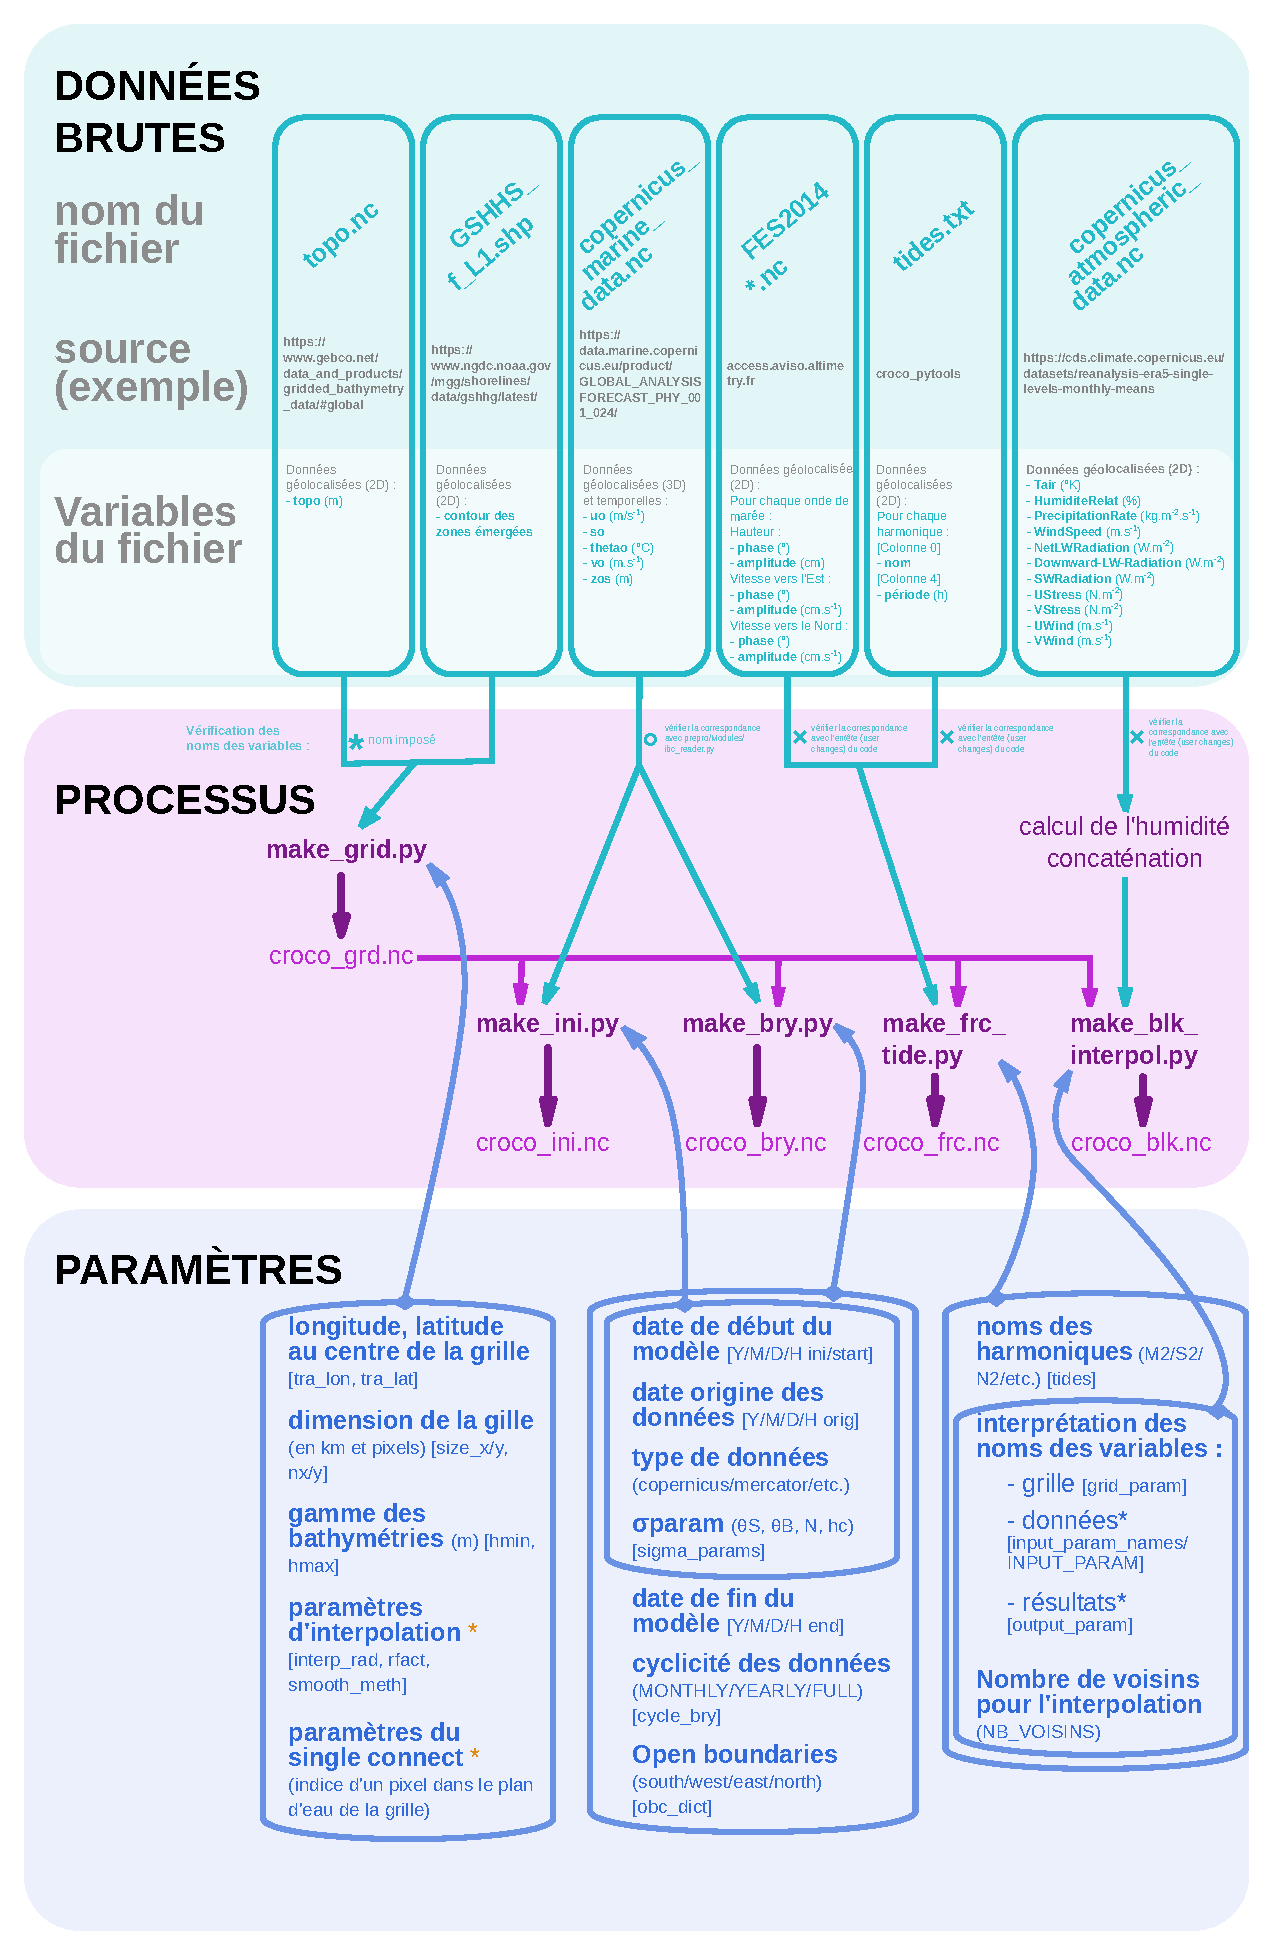
\includegraphics[scale=0.35]{../images/workflow/graphe_data_process_mere.pdf}
        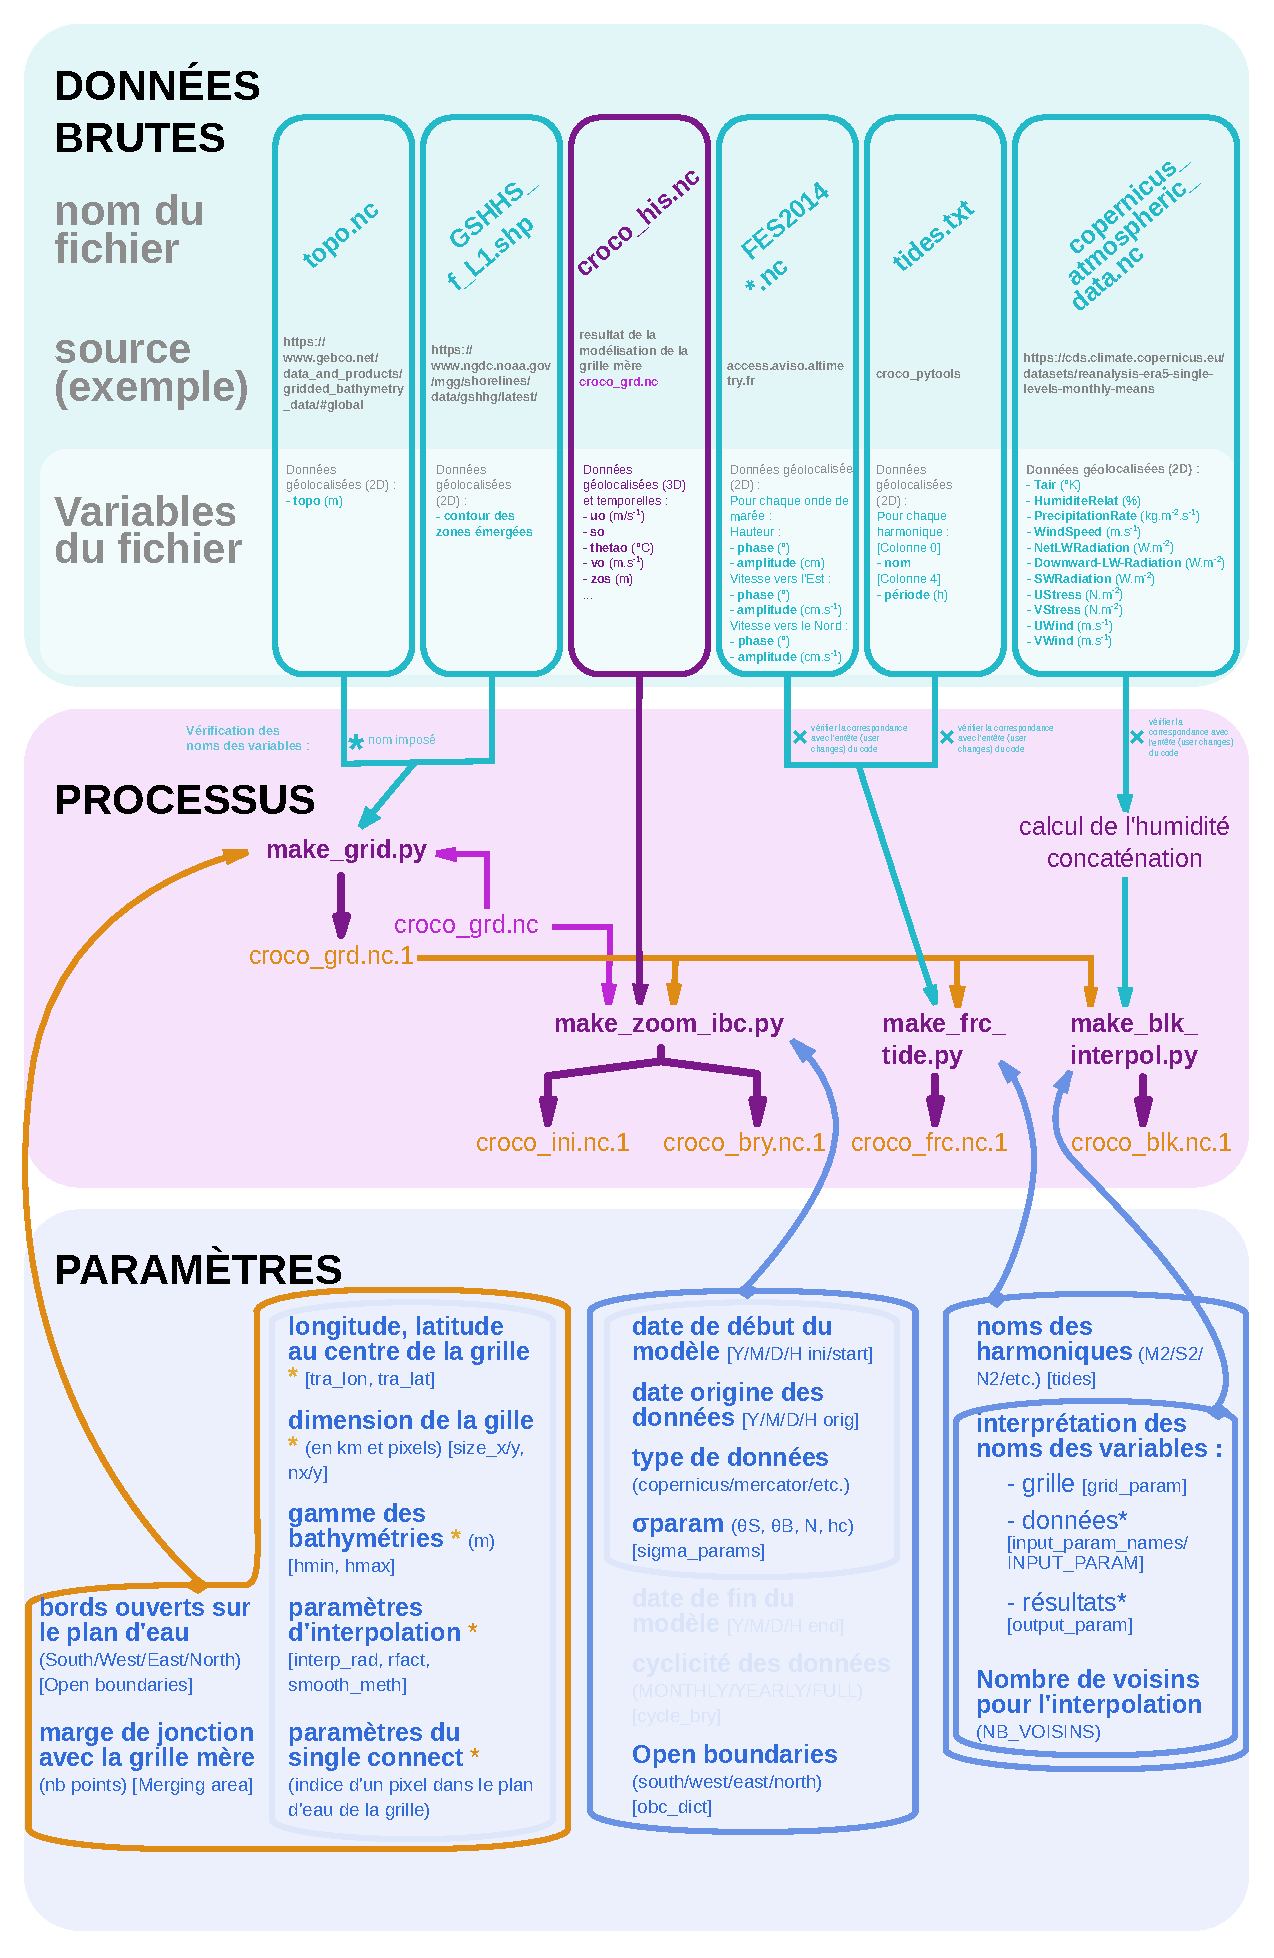
\includegraphics[scale=0.35]{../images/workflow/graphe_data_process_fille_zoom.pdf}
        \caption{
            \textbf{Pré-traitement avec les croco\_pytools pour une grille simple ({\color{workColor}mère}) à gauche et pour une sous-grille imbriquée ({\color{orange}fille}) à droite.}
            \\Les paramètres marqués d'une {\color{paramColor}astérisque (*) bleue} sont ceux qui doivent être modifiés en fonction du code pour lesquels ils sont utilisés (\textit{make\_frc\_tide.py} ou \textit{make\_blk\_interpol.py}).
            Les paramètres marqués d'une {\color{orange}astérisque (*) orange} sont des paramètres qui ont la même signification pour la grille mère et pour la grille fille mais leur valeur peut être différente pour chaque grille.
            Dans les données brutes de la grille fille, {\color{outputColor}croco\_his.nc} provient de l'exécution du modèle CROCO sur la grille mère {\color{workColor}croco\_grd.nc}.
            La signification des paramètres cités dans la figure est détaillée en Annexes.
        }
        \label{fig:workflow_prepro_main}
    \end{center}
\end{figure}

\subsubsection{La gestion de plusieurs grilles CROCO}
\label{subsub:gestion_multigrid}
D'autre part, les CROCO Pytools permettent la préparation de deux types de grilles emboîtées (Offline Zoom et AGRIF)

La méthode d'emboîtement des grilles AGRIF était préférée.
En effet, elle simplifie la modélisation du côté de l'utilisateur·ice qui n'a besoin de mettre en place et de démarrer le modèle qu'une unique fois pour obtenir les résultats de haute résolution des grilles filles.
D'autre part, elle a plus de chances de mieux représenter la réalité grâce à son fonctionnement en aller retour entre les grilles.

Toutefois, cette méthode a été abandonnée durant le stage car il est apparu, pendant les phases de test, que
(à lister... trop de dépendances et de contraintes sur les données utilisées).
Ainsi, c'est la méthode Offline zoom qui est utilisée pour la suite du rapport.

Chaque grille CROCO, pour être utilisée par le modèle, doit être liée à d'autres fichiers de données qui permettent l'initialisation et la mise en mouvement de la masse d'eau. Ces fichiers sont décrits dans les paragraphes suivants.

\subsubsection{La génération des données d'entrée}
\label{generation donnees entrée}
Les outils de pré-traitement originaux n'ont été utilisés que pour la génération des conditions initiales et au bord.
Les deux fichiers de forçage par la marrée et atmosphériques \ref{subsub:forcages_atm} ont été générés à partir de données brutes par deux scripts Python développés dans le cadre du stage.
En effet, les croco\_pytools associés à ces forçages n'étaient pas existants ou pas fonctionnels avec nos données.

\textbf{Les conditions initiales}\\
\label{par:cond_init}
Le fichier "croco\_ini.nc" contient notamment des données comme la température, la salinité, et la hauteur de la surface de l'eau. Ces données couvrent chaque maille de la grille CROCO et correspondent aux paramètres physiques de la zone au début de la modélisation.

\textbf{Les conditions aux bordures}\\
\label{par:cond_bords}
Le fichier "croco\_bry.nc" contient notamment les données comme la température, la salinité et éventuellement la hauteur d'eau et les vitesses des courants. Ces données couvrent seulement les bords extérieurs de la grille CROCO sur toute la durée temporelle de la modélisation.

\textbf{Les forçages par la marrée}\\
\label{par:forcages_marree}
Le premier script permet de générer un fichier de marrée pour CROCO à partir des données des modèles TPXO10 ou FES2014.
Dans ce script, les amplitudes et phases des vitesses des ondes de marée sont transformées en ellipse de périodicité selon les formules utilisée dans le croco\_pytool de référence,
$$SemiMajAxis = \abs{wp}+\abs{wm}$$
$$Eccentricity = \frac{\abs{wp}+\abs{wm}}{\abs{wp}-\abs{wm}}$$
$$Inclinaison = \frac{arg(wm)+arg(wp)}{2\pi}.180$$
$$PhaseAngle =  \frac{arg(wm)-arg(wp)}{2\pi}.180$$
avec 
\begin{equation*}
    wp = \frac{u*+j.v*}{2}
    \quad\mathrm{et}\quad 
    \overline{wm} = \frac{u*-j.v*}{2}
\end{equation*}
avec
\begin{equation*}u* = \exp(\frac{\pi PhaseU}{180}.(-1j)).AmplU 
    \quad\mathrm{et}\quad 
    v* = \exp(\frac{\pi PhaseV}{180}.(-1j)).AmplV
\end{equation*}
avec $PhaseU$, $PhaseV$, $AmpleU$, $AmplV$ les phases et amplitudes des composantes respectivement Sud-Ouest et Nord-Sud de la vitesse d'une onde de marée.

\textbf{les forçages atmosphériques}\\
\label{par:forcages_atm}
Le second génère un fichier de conditions atmosphériques en surface de l'eau à partir des données issues de Copernicus notamment.
Au préalable, les valeurs d'humidité relative $RH$ sont calculées et stockées dans une nouvelle variable selon la méthode décrite par \cite{humidity_formulation} en considérant une température entre $-20$ et $+50°C$ : $$RH = 10^{7,591386.(\frac{T_{dewpt}}{T_{dewpt}+240,7263}-\frac{T}{T+240,7263})}$$
avec $T_{dewpt}$ la température du point de rosée de l'air à $2m$ au dessus de la surface de l'eau et $T$ la température de l'air à la même altitude.


\subsection{Données de terrain - Le projet PROTEC}
\label{sub:protec}

Le "Projet de Territoire : Anse du Cul-de-Loup" (PROTEC) s'est déroulé de juin 2022 à juin 2024. Financé par l'Agence de l'Eau Seine-Normandie (AESN), ce programme de recherche était sous la responsabilité de G. Gregoire (MCF au Cnam/Intechmer) et a intéressé plusieurs autres membres de l'équipe du Cnam/Intechmer. L'objectif de PROTEC a été de dresser un état des lieux environnementale de l'anse du Cul-du-Loup, principalement sur les aspects en relations avec les sédiments, leur dynamique actuelle et passée (Fig. \ref{fig:sed-adcl}).

\begin{figure}[!h]
    \centering
    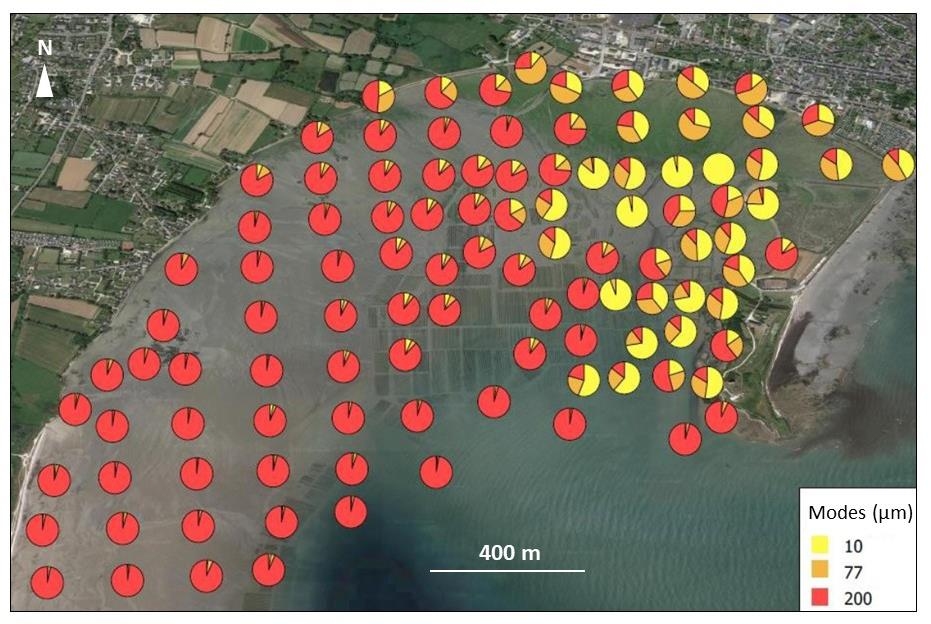
\includegraphics[width=0.8\linewidth]{../images/sed_adcl_protec.png}
    \caption[Sédiment de l'anse du Cul-de-Loup]{Pourcentages relatif des principales fractions granulométriques dans des échantillons sédimentaires de surface prélevés dans l'anse du Cul-de-Loup (jaune - 10 $\mu$m, orange - 77 $\mu$m, rouge - 200 $\mu$m).}
    \label{fig:sed-adcl}
\end{figure}


\subsection{Post processing}
\label{sub:postpro}
à voir, détailler :
\begin{itemize}
    \item l'écriture de scripts pour extraire le point le plus proches,
    \item les choix pour les interpolations (closest neighbor),
    \item les REQM utilisés (RMSEDEI).
\end{itemize}


\newpage
\section{RÉSULTATS}
\label{sec:resultats}

%{\color{lightgrey}
%Mettre les résultats uniquement.
%}

\subsection{Le modèle "Anse du Cul-de-Loup"}
%{\color{lightgrey}
%    Grosse partie dans laquelle il va falloir expliquer les différentes étapes de mis en place du modèle ADCL (pour la mise en place non spécifique à la zone, partie précédente ?) détailler les paramètres choisis.
%}

La lecture de la documentation, des codes des CROCO Pytools et de fichiers d'exemple de sortie du pré-traitement Matlab ont permis de réaliser des choix pour le pré-traitement.
Ce dernier à aboutit à la préparation correcte des fichiers pour l'exécution du code CROCO.
Les choix qui ont été faits sont détaillés dans les parties suivantes.

\subsubsection{Données brutes utilisées}
Plusieurs types de fichiers de données brutes sont recherchées. L'ensemble de ces fichiers est représenté en Figure \ref{fig:workflow_prepro_main}.
La majorité des données proviennent des bases de données de Copernicus (marine ou climate).
Les données de marrée du modèle TPXO10 ont été testées, mais ce sont les résultats du modèle FES2014 qui ont finalement été retenus. (indiquer pourquoi ? meilleure résolution dans notre zone ?)

Pour la majorité de la surface couverte par la grille mère, les données de bathymétrie proviennent du GEBCO 2024.
Ces données sont continues dans l'espace.
Par ailleurs, la campagne PROTEC offre des données de haute résolution mais discontinues sur la zone de l'Anse du Cul-de-Loup.
Les données provenant de GEBCO et PROTEC sont donc fusionnées entre elles afin d'obtenir une cartographie bathymétrique de haute résolution dans les zones où les données le permettent.

Enfin, les fichier vectoriels géo-référencés qui définissent le trait de côte proviennent de la National Oceanic and Atmospheric Administration (NOAA).
Ces données vectorielles sont corrigées par les données de la campagne PROTEC qui sont plus précises mais qui couvrent seulement le Nord du Cotentin.

Une fois ces données acquises, il convient de générer la grille du modèle ainsi que ses fichier d'initialisation et de contraintes au limites.
Les paramètres de cette grille sont utilisés par les codes de pré-traitement pour transformer les données brutes en données utilisables par CROCO.

\subsubsection{Paramètres généraux choisis}
{\color{lightgrey}
    Paramètres de la grille (étendue, localisation, résolution horizontale et verticale, etc.), choix du LES.
}

Les paramètres généraux sont majoritairement déterminés par l'utilisateur·ice lors de l'exécution du CROCO Pytool de création de la grille.
Cette grille est fondamentale au fonctionnement de CROCO, elle détermine en quels point sont résolues les équations du modèle. Ses principales propriétés sont :

\begin{itemize}
    \item sur chaque plan horizontal, la grille couvre la même zone rectangulaire sur Terre, à l'exception des zones émergées,
    \item les espacement en latitude et longitude des mailles sont réguliers.
\end{itemize}

D'autre part, les propriétés verticales ($\sigma_{param}$) de la modélisation sont d'une grande importance, notamment pour la qualité de la résolution des turbulences et des mélanges avec la surface du plan d'eau.
Ces propriétés ne sont pas directement déterminées dans le fichier contenant la grille CROCO.
Toutefois, les $\sigma_{param}$ doivent être fixés par l'utilisateur·ice dans les différents CROCO Pytools de génération des conditions initiales et aux limites, comme représenté dans la Figure \ref{fig:workflow_prepro_main}.

\begin{itemize}
    \item le nombre de points alignés verticalement est constant quelque soit la bathymétrie dans le plan d'eau,
    \item les espacements verticaux entre les mailles de la grille sont variables. Ils respectent les paramètre $\theta_s$, $\theta_b$, $hc$ et $n$ qui imposent des répartitions verticales respectant la bathymétrie en chaque point comme illustré par la Figure \ref{fig:vertical_resolution}.
\end{itemize}

\begin{figure}[h!]
    \centering
    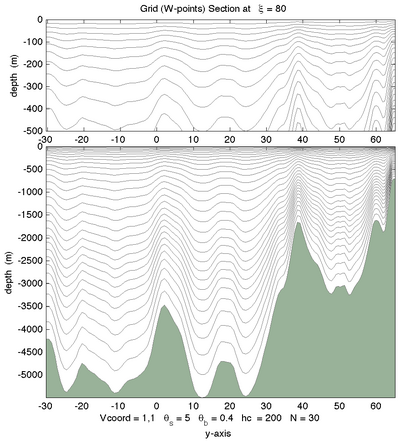
\includegraphics{../images/vcoord_ex1.png}
    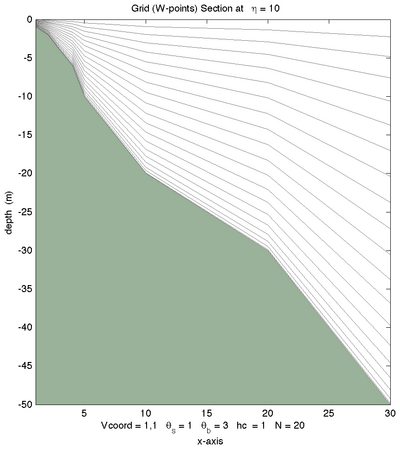
\includegraphics{../images/vcoord_ex5.png}
    \caption{\textbf{Exemples de résolutions verticales variables déterminées par la topographie et les paramètres  $\sigma_{param}$ entrés par l'utilisateur·ice.} \\
        À gauche, les paramètres choisis sont  $\protect\theta_s = 7$, $\protect\theta_b = 0.1$, à droite ils sont  $\protect\theta_s$ = 7, $\protect\theta_b = 3$.}
    % (source : https://croco-ocean.gitlabpages.inria.fr/, https://myroms.org/)
    \label{fig:vertical_resolution}
\end{figure}

Les paramètres entrés par l'utilisateur·ice fixent la localisation en latitude et longitude de la grille, sa résolution dans les trois dimensions de l'espace ainsi que le choix de la restriction de la modélisation à un seul plan d'eau.
De plus, la grille est générée en utilisant les données brutes de bathymétrie et de trait de côte, comme décrites dans la partie précédente.

La localisation et l'étendue spatiale de la grille sont choisies afin que ses faces ouvertes sur le plan d'eau soient le moins possible recoupées par des zones émergées.

\subsubsection{Augmentation de la résolution}
{\color{lightgrey}
    Nombre et paramètres des grilles imbriquées
}

La zone d'étude a un rayon d'une dizaine de kilomètre et la résolution des données attendues est d'au moins quelques dizaines de mètre.
Toutefois, les données brutes (les modèles de marrées et les données générales marines et atmosphérique) qui sont utilisées pour fixer les conditions initiales et aux limites pour un modèle dans cette zone ont une résolution largement inférieure à celle attendue en sortie de modèle.
Il est donc intéressant de mettre en place un ensemble de modélisations en grilles emboîtées afin de décrire correctement les courants autour du Nord du Cotentin.
L'imbrication successive des grilles permet d'aboutir à la modélisation plus réaliste et stable numériquement d'une zone restreinte à l'Anse du Cul-de-Loup.
Trois grilles emboîtées ont ainsi été réalisées ici, elles sont illustrées en Figure \ref{fig:imbrication}.

\begin{figure}[h!]
    \centering
    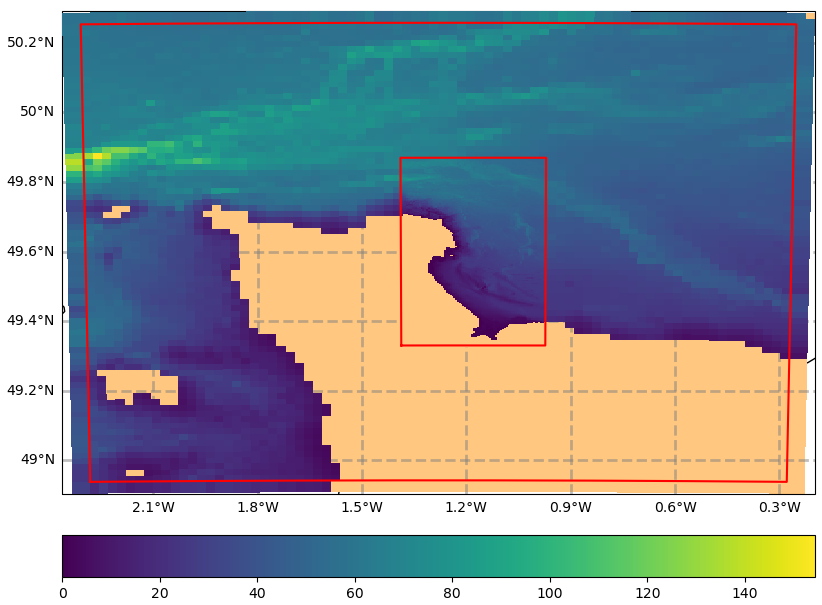
\includegraphics[scale=0.4]{../images/croco_grd.nc.1_V2.png}
    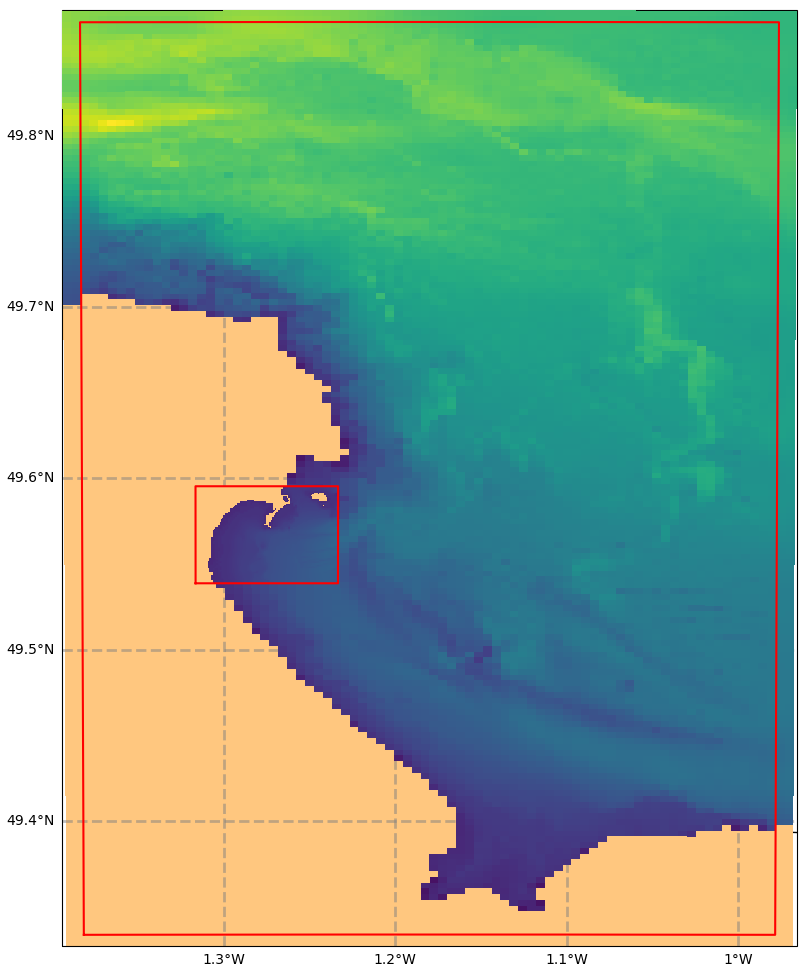
\includegraphics[scale=0.27]{../images/croco_grd.nc.2_V2.png}
    \caption{
        \textbf{Visualisation des grilles emboîtées choisies pour la modélisation de l'Anse du Cul-de-Loup.}
        À gauche, la grille mère est délimitée par le grand rectangle rouge, sa grille fille est délimitée par le petit rectangle rouge.
        À droite, la même grille fille correspond au grand rectangle, elle est mère de la grille petite-fille délimitée par le petit rectangle rouge.
        Les pixels oranges sont les maille considérées comme obligatoirement émergées. Ainsi, les équations du modèle n'y seront par résolues.
        Les autres couleurs (du bleu au jaune) représentent la bathymétrie dont les échelles respectives sont représentées en dessous de chaque graphique.
    }
    \label{fig:imbrication}
\end{figure}

La position des grilles emboîtées est déterminée selon deux règles :
\begin{itemize}
    \item les bords de la grille fille doivent être assez loin des bords ouverts sur le plan d'eau de la grille mère, leur centre est donc généralement proche,
    \item au niveau de l'intersection entre les bords d'une grille et le tracé de la côte, ce dernier doit être le plus simple possible, c'est à dire de préférence rectiligne en Nord-Sud ou Est-Ouest.
    De plus, pour les grilles filles, le tracé de la côte au niveau des bords doit être aligné avec le tracé de la côte de la grille mère.
\end{itemize}

\subsection{Résultats (sortie de modèle)}

Sorties selon les choix de modélisation:
\begin{itemize}
    \item mode hydro (RANS, LES, etc.) (à voir)
    \item effet de l'atmosphère (bulk / climato)
    \item couplage avec les vagues (WaveWatch-III) (pas encore fait)
\end{itemize}

Visualisation : snapshots représentatifs de la marée, zoom sur des zones dynamiques

Comparaisons : différences, variations de l'écart type

\newpage

\section{DISCUSSION}
\label{sec:discussion}

Comparaison des résultats du modèle avec les mesures de terrain: graphiques, indicateurs de qualité (RMSE, etc.)

\newpage

\section{CONCLUSION}
\label{sec:conclusion}

Ca sera fait à la fin ou presque


\newpage
\section*{ANNEXES}

\section{schémas numériques}
\subsection{Shema WENO de cinquième ordre (Weighted Essentially Non-Oscillatory scheme)}\label{WENO}
Les variables sont disposées en C-grille d'Arakawa.
Les valeurs des traceurs sont notées $q_i$ et les vitesses $u_i$.
Dans le cadre de ce schémas d'advection, trois valeurs aux interfaces sont évaluées en se utilisant trois stencils différents. Une moyenne non linéaire entre ces trois valeurs est utilisée comme suit pour déterminer la valeur calculée :
$$\tilde{q}_{k-\frac{1}{2}} = a_1k-\frac{1}{2}^{(1)} + a_2k-\frac{1}{2}^{(2)} + a_2k-\frac{1}{2}^{(2)}$$
Les constantes de pondération sont définies selon les règles suivantes :
\begin{enumerate}
    \item $\sum_{j=0}^{2}a_j = 1$,
    \item propriété ENO (Essentially Non Oscillatory),
    \item cinquième ordre à condition que q(x) soit peut rugueux.
\end{enumerate}
C'est un schéma à variation bornée (TBV, Total variation Bounded).
source : \cite{schemas_advection}


\section{MATÉRIELS ET MÉTHODES}

\subsection{Le code de calcul CROCO}

mettre les principes généraux de CROCO (origine, type de modèle, etc...)

+ organisation des fichiers


\color{darkgrey}
\dirtree{%
    .0 ~/\DTcomment{le chemin peut être différent pour PATH-TO-CROCO/ et PATH-TO-CONFIG/}.
    .1 PATH-TO-CROCO/.
    .2 croco/\DTcomment{dossier généré par l'installation de croco}.
    .3 OCEAN/.
    .3 SCRIPTS/.
    .3 MUSTANG/.
    .3 AGRIF/.
    .3 create\_config.bash.
    .3 version.txt.
    .3 REANDME.md.
    .3 CHANGELOG.md.
    %
    .2 croco\_pytools/\DTcomment{dossier généré par l'installation des outils python (croco\_pytools)}.
    .3 prepro/.
    .4 Modules/.
    .5 tides.txt.
    .4 Readers/.
    .5 ibc\_reader.py.
    .5 topo\_reader.py.
    .4 make\_grid.py.
    .4 make\_ini.py.
    .4 make\_bry.py.
    .3 make\_blk\_interpol.py.
    .3 make\_frc\_tide.py.
    %
    .1 PATH-TO-CONFIGS/.
    .2 CONFIGS/\DTcomment{dossier pouvant être généré avec create\_config.bash (modifié selon la partie \ref{create_config})}.
    .3 CONFIG-NAME/.
    .4 datasets/.
    .5 Bry/.
    .6 AVISO/.
    .7 FES2014*.nc.
    .6 ../Ini/copernicus\_marine\_data.nc.link.
    .5 Bulk/.
    .6 cpernicus\_atmospheric\_data.nc.
    .5 gshhs/.
    .6 GSHHS\_f\_L1.shp.
    .5 Ini/.
    .6 copernicus\_marine\_data.nc.
    .5 Topo/.
    .6 topo.nc.
    .4 preproOUTPUT/.
    .4 cppdefs.h.
    .4 param.h.
    .4 jobcomp.
    .4 croco.in.
    %
}
\color{black}

\subsubsection{Processus généraux}

\textbf{Installation}

Explication de l'installation des pytools, de croco et de l'activation de l'environnement Anaconda/Miniconda \textit{croco\_pyenv}.

\begin{codeEnv}{installation de croco}
    \begin{lstlisting}[language=bash]
        # en se placant dans PATH-TO-CROCO/
        git clone --branch v2.0.1 https://gitlab.inria.fr/croco-ocean/croco.git croco-v2.0.1
    \end{lstlisting}
\end{codeEnv}

\begin{codeEnv}{installation de miniConda}
    \begin{lstlisting}[language=bash]
        wget https://repo.anaconda.com/miniconda/Miniconda3-latest-Linux-x86_64.sh
        sudo chmod +x Miniconda3-latest-Linux-x86_64.sh
        bash Miniconda3-latest-Linux-x86_64.sh -p $HOME/miniconda3
        source $HOME/miniconda3/bin/activate
        conda init
    \end{lstlisting}
\end{codeEnv}

\begin{codeEnv}{installation des croco\_pytools}
    \begin{lstlisting}[language=bash]
        # en se placant dans PATH-TO-CROCO/
        git clone --branch release https://gitlab.inria.fr/croco-ocean/croco_pytools.git
        cd croco_pytools/prepro/
        # conda activate croco\_pyenv
        python3 install.py
        > Do you want to install conda environment? [y,[n]]: y
        > Do you want to compile fortran tools? y,[n]: y
    \end{lstlisting}
\end{codeEnv}

Une fois croco et les croco\_pytools installés, l'achitecture de la configuration doit être générée. Nativement, croco contient un fichier \textit{create\_config.bash} qui effetue ce travail. Toutefois, comme l'architecture choisie pour ce rapport est différente de celle de référence, un nouveau fichier \textit{create\_config.bash} a été écrit, son contenu est défini ci-après.

\begin{codeEnv}{\textbf{contenu de \textit{create\_config.bash} adapté à l’architecture choisie pour ce rapport}}\label{create_config}
    \begin{lstlisting}[language=bash]
        # croco source directory
        # ---------------------
        CROCO_DIR=~/PATH-TO-CROCO/croco

        # Home and Work configuration directories
        # ---------------------------------------
        MY_CONFIG_HOME=~/PATH-TO-CONFIGS/CONFIGS

        # croco_tools directory for matlab tools
        # ---------------------
        # TOOLS_DIR=~/PATH-TO-CROCO/croco_pytools
        # For pre-processing WITH MATLAB:
        #cp ${TOOLS_DIR}/crocotools_param.m ${MY_CONFIG_HOME}/${MY_CONFIG_NAME}/
        #cp ${TOOLS_DIR}/start.m ${MY_CONFIG_HOME}/${MY_CONFIG_NAME}/

        # Configuration name
        # ------------------
        MY_CONFIG_NAME=CONFIG-NAME  # put the name you want

        # For configuration initialisaiton
        mkdir ${MY_CONFIG_HOME}/${MY_CONFIG_NAME}
        mkdir ${MY_CONFIG_HOME}/${MY_CONFIG_NAME}/datasets
        mkdir ${MY_CONFIG_HOME}/${MY_CONFIG_NAME}/datasets/Bry
        mkdir ${MY_CONFIG_HOME}/${MY_CONFIG_NAME}/datasets/Bulk
        mkdir ${MY_CONFIG_HOME}/${MY_CONFIG_NAME}/datasets/gshhs
        mkdir ${MY_CONFIG_HOME}/${MY_CONFIG_NAME}/datasets/Ini
        mkdir ${MY_CONFIG_HOME}/${MY_CONFIG_NAME}/datasets/Topo


        # For pre-processing WITH PYTHON :
        mkdir ${MY_CONFIG_HOME}/${MY_CONFIG_NAME}/preproOUTPUT

        # For CROCO compiling
        cp ${CROCO_DIR}/OCEAN/cppdefs.h ${MY_CONFIG_HOME}/${MY_CONFIG_NAME}/
        cp ${CROCO_DIR}/OCEAN/param.h ${MY_CONFIG_HOME}/${MY_CONFIG_NAME}/
        cp ${CROCO_DIR}/OCEAN/jobcomp ${MY_CONFIG_HOME}/${MY_CONFIG_NAME}/

        # For running
        cp ${CROCO_DIR}/OCEAN/croco.in ${MY_CONFIG_HOME}/${MY_CONFIG_NAME}/

    \end{lstlisting}
\end{codeEnv}

\textbf{Plan général des étapes}



Le schéma Figure\ref{fig:workflow_simple} résume les étapes de décision et de traitement de données et d'exécution de codes décrit ci-après.

\begin{processEnv}{\textbf{Plan des processus généraux à suivre pour mettre en place un modèle fonctionnel}}

    {\color{paramColor}\textbf{Paramètres du modèle}}

    Avant de rechercher les données qui seraient trop lourdes à télécharger à l'échelle globale, il convient de déterminer les propriétés principales de la zone d'étude et de son modèle. Ces paramètres sont :

    \begin{enumerate}
        \item les latitudes et longitudes du centre de la zone d'étude totale,
        \item l'étendue en kilomètres de la zone d'étude dans le sens de la latitude et de la longitude,
        \item la gamme de bathymétrie que doit couvrir le modèle (minimum et maximum),
        \item les paramètres d'interpolation qui doivent être utilisés pour les données de bathymétrie,
        \item les coordonnées d'un point de la grille se trouvant dans le plan d'eau d'intérêt si le modèle ne doit tourner que sur un plan d'eau,
        \item les dates de début et de fin de la modélisation,
        \item les valeurs associées à la répartition des mailles verticales de la grille. Leur nombre $N$ doit aussi être déterminé.
    \end{enumerate}


    {\color{dataColor}\textbf{Données en entrée}}

    En entrée, les données brutes nécessaires doivent toujours couvrir spatialement l'intégralité de la zone d'étude. Elles doivent être placées dans le dossier PATH-TO-CONFIGS/CONFIGS/CONFIG-NAME/datasets/.
    Elles sont :

    \begin{enumerate}
        \item la bathymétrie {\color{darkgrey}[topo.nc]} couvrant au moins la zone d'étude,
        \item le masque côtier {\color{darkgrey}[GSHHS\_f\_L1.shp]} comprenant au moins les côtes de la zone d'étude,
        \item les données marines {\color{darkgrey}[copernicus\_marine\_data.nc]} couvrant une zone la plus large possible autour et comprenant la zone d'étude. Ces données doivent aussi couvrir le plus finement possible la gamme temporelle mentionnée dans la section précédente,
        \item les données issues d'un modèle global ou local de marée, par exemple TPXO10 ou FES2014 {\color{darkgrey}[FES2014*.nc]} incluant des données de hauteur d'eau et de courant pour les différentes fréquences de vagues de marrée (M2, S2, N2, K2, K1, O1, P1, Q1, MF, MM,...)
        \item le fichier texte présent nativement dans les croco\_pytools {\color{darkgrey}[tides.txt]} contenant les noms et les périodes des différentes harmoniques des vagues de marrée.
        \item les données atmosphériques {\color{darkgrey}[copernicus\_atmospheric\_data.nc]} couvrant une zone large autour et comprenant la zone d'étude. Ces données doivent couvrir le plus finement possible la gamme temporelle mentionnée dans la section précédente.
    \end{enumerate}

    Les {\color{paramColor}\textbf{paramètres}} qu'il conviendra de récupérer dans la documentation des données de forçage (initial et aux limites) sont :

    \begin{enumerate}
        \item les dates qui correspondent à l'origine du temps donné dans les fichiers téléchargées (généralement 1970/01/01),
        \item la nomenclature des variables devra aussi être vérifiée en fonction du contenu de \textit{croco\_pytools/prepro/Readers/ibc\_reader.py},
        \item l'orientation des limites de la grille ouvertes dans le plan d'eau,
        \item la cyclicité potentielle des données entrées.
    \end{enumerate}

    {\color{workColor}\textbf{Pré-processing}}

    Le pré-processing des données brutes n'est détaillé ici que pour les croco\_pytools. Les outils Matlab ne sont pas abordés.

    \textbf{- modifications basiques des fichiers netCDF}

    Certaines modifications peuvent êtres préférablement réalisées avant d'utiliser les outils de pré-processing. Ces modifications peuvent être effectuées en utilisant la librairie NCO de traitement des fichiers netCDF

    \begin{codeEnv}{\textbf{Changer le nom d'une variables du fichier}}
        \begin{lstlisting}[language=bash]
            # renome la variable t2m en HR
            nco chname,t2m,HR
        \end{lstlisting}
    \end{codeEnv}

    Cette commande n'est pas obligatoire car les fichiers "ibc\_reader.py", "make\_frc\_tide.py" et "make\_blk\_interpol.py" peuvent être adaptés à la main.
    La commande reste utile si on souhaite dupliquer une variable (La marche à suivre est : dupliquer un fichier en in1.nc et in2.nc, puis renommer la variable A en A2 du fichier nc2.nc, puis concaténer les fichiers in1.nc et in2.nc. Le fichier de sortie contient alors les deux variables identiques A et A2).

    \begin{codeEnv}{\textbf{Rognage des données selon une dimension}}
        \begin{lstlisting}[language=bash]
            # rogne selon les indices de la dimension time et
            # selon les valeurs des dimensions longitude et latitude
            ncks -d time,240,359 -d longitude,-2.,3. -d latitude,48.,50. in.nc out.nc
        \end{lstlisting}
    \end{codeEnv}

    Si des des entiers (exemple : 40) sont donnés pour la gamme à restreindre d'une dimension, ces valeurs sont interprétées comme les \textbf{indices} des dimensions minimum et maximum. Si des décimaux (exemple : 40.) sont donnés, les valeurs sont interprétées comme les \textbf{valeurs }minimales et maximales des dimensions.

    \begin{codeEnv}{\textbf{Concaténation de plusieurs fichiers selon les dimensions communes}}
        \begin{lstlisting}[language=bash]
            # concatene tous les fichiers data_*.nc en un fichier data_tot_calc.nc
            ncks -h -A raw_download/data_*.nc data_tot_calc.nc
        \end{lstlisting}
    \end{codeEnv}

    \begin{codeEnv}{\textbf{Effectuer une opération arithmétique sur plusieurs variables du fichier}}
        \begin{lstlisting}[language=bash]
            # calcule et stocke dans RH les valeurs d'humidite relative selon
            # les valeurs des variables d2m (temperature du point de rosee)
            # et t2m (temperature)
            ncap2 -s 'RH=10^(7.591386*(d2m/(d2m+240.7263)-t2m/(t2m+240.7263)))'\
            in.nc out.nc
        \end{lstlisting}
    \end{codeEnv}

    \begin{codeEnv}{\textbf{Effectuer une opération arithmétique sur plusieurs variables du fichier}}
        \begin{lstlisting}[language=bash]
            # change a "new attribute str value" la valeur de l'attribut "attribute"
            # de la variable "variable" du fichier "in.nc"
            ncatted -a attribute,variable,o,c,"new attribute str value" in.nc
        \end{lstlisting}
    \end{codeEnv}

    \textbf{- Génération de la grille}

    La grille \textit{croco\_grd.nc} est la base des prochaines actions de pré-processing ainsi que du modèle. Elle contient toutes les données relatives aux coordonnées de chaque maille de la grille sur laquelle le va travailler, ainsi que les données de bathymétrie, un paramètre de Coriolis et les coordonnées curvilinéaires des mailles.

    \begin{codeEnv}{\textbf{générer la grille en mode graphique}}
        \begin{lstlisting}[language=bash]
            # dans PATH-TO-CROCO/croco_pytools/prepro/
            python3 make_grid.py
            > Do you want to use interactive grid maker ?
            > (e.g., for grid rotation or parameter adjustments) : y,[n] y
        \end{lstlisting}
    \end{codeEnv}

    Dans la fenêtre graphique, les champs doivent être modifiés pour correspondre aux paramètres voulus. Ils peuvent être aussi déterminés et choisis par tâtonnement en utilisant les boutons \textit{Compute grid} et \textit{Compute smoothing} successivement.

    Les valeurs utilisées pour modéliser le Cotentin (France) ainsi que les visualisation proposées sont présentées en Figure \ref{make_grid_main}.

    Une fois la grille souhaitée obtenue, la sauvegarder en utilisant le bouton \textit{Save grid}.

    \textbf{- Génération des fichiers de données}

    Tous les codes de pré-processing suivants peuvent être exécutés dans n'importe quel ordre en se plaçant dans le répertoire du code voulu et en indiquant l'intitulé de ce code dans la commande:

    \begin{codeEnv}{\textbf{exécuter un code de pré-pocessing}}
        \begin{lstlisting}[language=bash]
            python3 <name_of_the_pre-pro_code>.py
        \end{lstlisting}
    \end{codeEnv}

    Au début de chaque code, une partie dans l'entête encadrée par \lstinline[language=python]|###...## USER CHANGES ###...###| et \lstinline[language=python]|###...## end USER CHANGES ###...###| doit être relue pour indiquer les bon paramètres ainsi que les noms et registres des fichiers de données brutes nécessaires.

    Les codes devant être exécutés sont dans le répertoire \textit{croco\_pytools/} :

    \begin{enumerate}
        \item \textit{prepro/make\_ini.py} génération des conditions initiales à partir des données marines,
        \item \textit{prepro/make\_bry.py} génération des conditions (de pression, température, salinité, etc.) aux bords ouverts sur le plan d'eau de la grille, à partir des données marines,
        \item \textit{make\_frc\_tide.py} génération des conditions de forçage par les modèles de marrées pour les bords ouverts sur le plan d'eau de la grille, à partir des données issues d'un modèle de marée,
        \item \textit{make\_blk\_interpol.py} génération des conditions de forçage atmosphériques à la surface du plan d'eau sur l'ensemble de la grille, à partir des données atmosphériques.
    \end{enumerate}

    Ces codes vont respectivement générer les fichiers de données :

    \begin{enumerate}
        \item \textit{croco\_ini.py}
        \item \textit{croco\_bry.py}
        \item \textit{croco\_frc.py}
        \item \textit{croco\_blk.py}
    \end{enumerate}

    Le schéma XXX détaille les dépendances de fichiers et les paramètres à spécifier pour chaque code de pré-processing.

    Attention, à partir de deux grilles filles, il convient de corriger manuellement le fichier AGRIF\_FixedGrids.in.

    {\color{workColor}\textbf{Modélisation}}

    \textbf{- Modification des fichiers de compilation}

    Les fichiers qui doivent être modifiés (ou écrits) sont :

    \begin{itemize}
        \item croco.in (+ croco.in.n avec n allant de 1 au nombre de grilles enfants)
        \item param.h
        \item cppdefs.h
        \item jobcomp
    \end{itemize}

    \textbf{- Compilation du modèle}

    \begin{codeEnv}{\textbf{commande pour compiler le code CROCO}}
        \begin{lstlisting}[language=bash]
            # dans PATH-TO-CONFIGS/CONFIGS/CONFIG-NAME/
            ./jobcomp
        \end{lstlisting}
    \end{codeEnv}

    \textbf{- Exécution du modèle}

    \begin{codeEnv}{\textbf{commande pour exécuter le code CROCO}}
        \begin{lstlisting}[language=bash]
            # dans PATH-TO-CONFIGS/CONFIGS/CONFIG-NAME/
            ./croco
        \end{lstlisting}
    \end{codeEnv}

    {\color{outputColor}\textbf{Fichiers de sortie}}

    La compilation du modèle produit les fichiers :

    \begin{itemize}
        \item de dossier Compile dans son intégralité,
        \item croco,
        \item ncjoin,
        \item partit,
        \item kRGB61.txt.1,
        \item kRGB61.txt
    \end{itemize}

\end{processEnv}
\begin{comment}
    \begin{codeEnv}{\textbf{Exemple de code Python}}
        \begin{lstlisting}[language=python]
            class MyClass(Yourclass):
            def __init__(self, my, yours):
            bla = '5 1 2 3 4'
            if 1 < 4:
            print bla # show in terminal
        \end{lstlisting}
    \end{codeEnv}
\end{comment}

\subsubsection{Détail des processus du pre-processing}
Un schéma détaillé de la marche à suivre pour générer les fichiers nécessaires au modèle à partir des données brutes, c'est à dire le pre-processing, est présenté en Figure \ref{fig:workflow_prepro_main}.
Les chemins de fichiers présentées dans le rapport correspondent à la nomenclature définie en section \ref{create_config}.


[LA SUITE EN ANNEXES ?]

\textbf{make\_grid.py}

L'entête du code \textit{make\_grid.py} doit être adaptée aux paramètres choisis et à l'emplacement des données.

\begin{codeEnv}{\textbf{modifications utilisateur·ice de make\_grid.py}}
    \begin{lstlisting}[language=python]
        #--- USER CHANGES ---------------------------------------------------------

        # Grid center [degree]
        tra_lon =  15 # Longitude of the grid center
        tra_lat = -32 # Latitude of the grid center

        # Grid size [km]
        size_x = 1556
        size_y = 1334

        # Grid number of points
        # Note: grid resolution is grid size / number of points
        nx = 39
        ny = 40

        # Grid rotation [degree]
        rot = 0

        # Smoothing parameters
        # (see online documentation for more details)
        hmin        = 50    # Minimum depth [m]
        hmax        = 6000  # Maximum depth [m]
        interp_rad  = 2     # Interpolation radius in number of points
        #                        (usually between 2 and 8)
        rfact       = 0.2   # Maximum r-fact to reach
        #                        (the lower it is, the smoother it will be)
        smooth_meth = 'lsmooth'  # Smoothing method ('smooth', 'lsmooth',
        #                           'lsmooth_legacy', 'lsmooth2', 'lsmooth1',
        #                           'cond_rx0_topo')

        # Topo/Bathy file
        topofile = 'PATH-TO-CONFIGS/CONFIGS/CONFIG-NAME/dataset/Topo/etopo2.nc'

        # Coastline file (for the mask)
        shp_file = 'PATH-TO-CONFIGS/CONFIGS/CONFIG-NAME/dataset/gshhs/GSHHS_i_L1.shp'

        # Single Connect [Mask water not connected to the main water body]
        sgl_connect=[False,20,20]  # point indices inside the main water body
        #                               (True or False)

        # Output grid file
        output_file="PATH-TO-CONFIGS/CONFIGS/CONFIG-NAME/preproOUTPUT/croco_grd.nc"

        #--- END USER CHANGES -----------------------------------------------------
    \end{lstlisting}
\end{codeEnv}
+ modifs en graphic mode si on souhaite générer des sous-grilles (AGRIF) voir Figure \ref{make_grid_main}.

\begin{figure}
    \begin{center}
        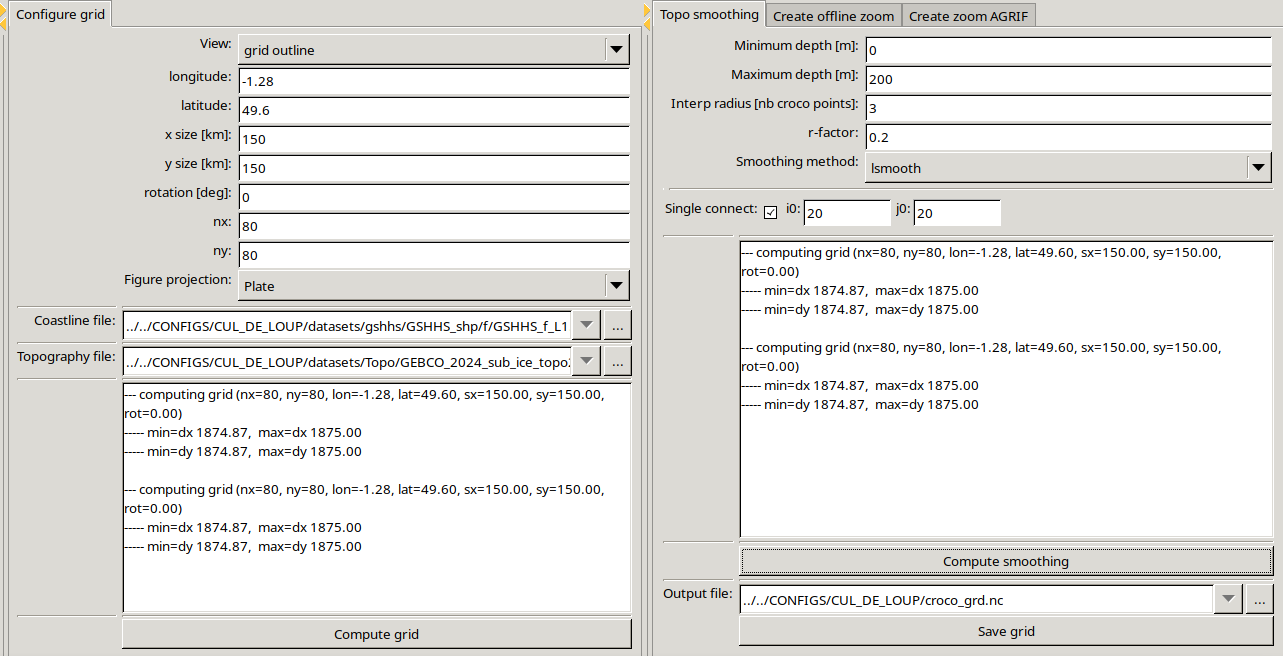
\includegraphics[scale=0.4]{../images/makegrid/parameters_main.png}

        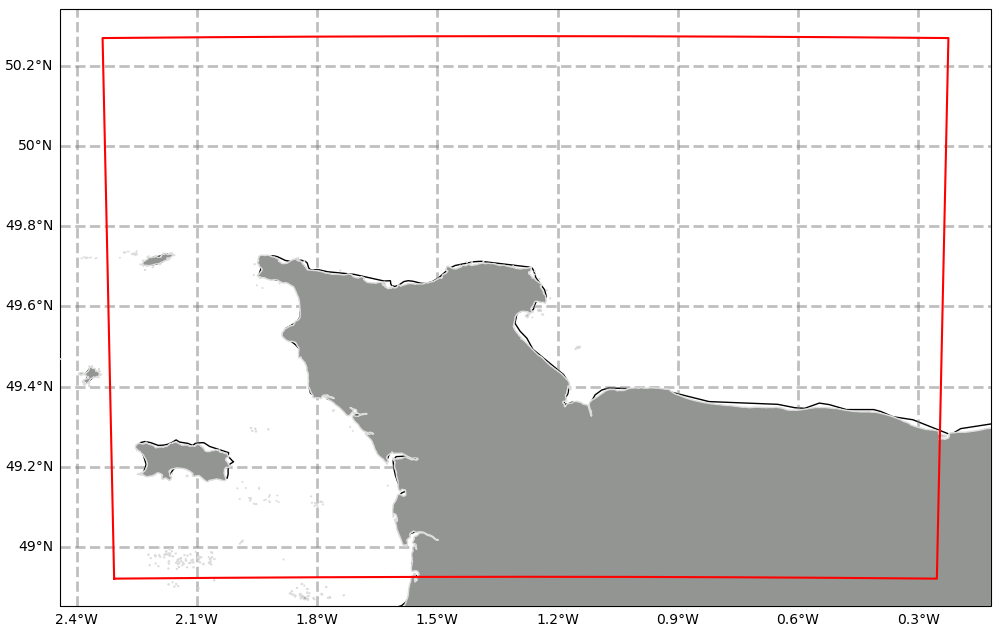
\includegraphics[scale=0.2]{../images/makegrid/config_main.png}
        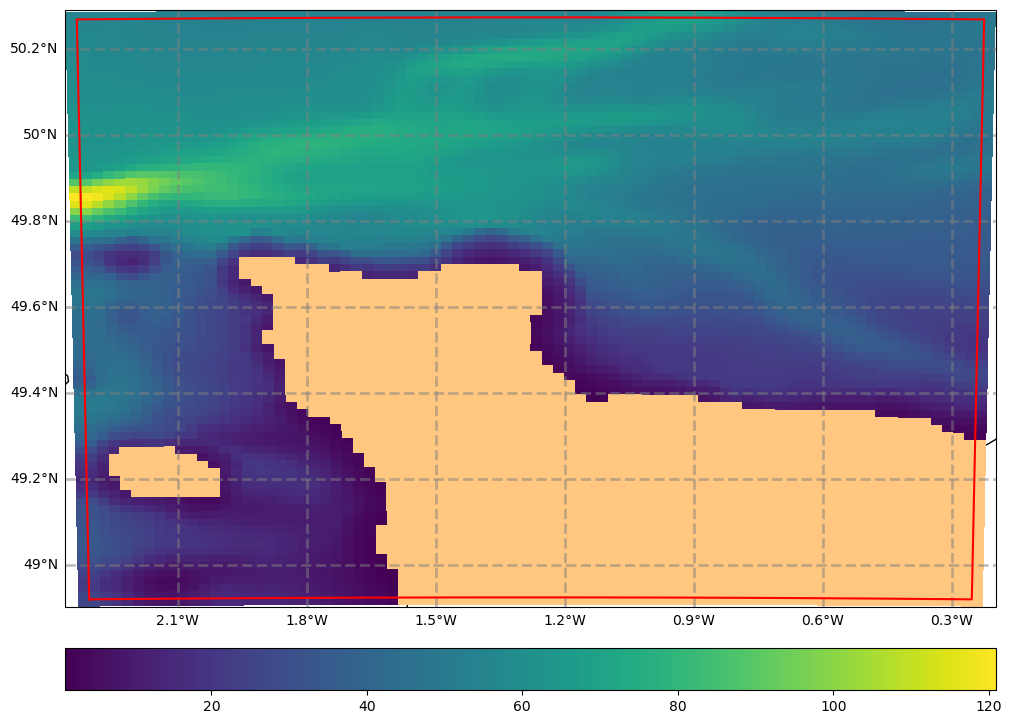
\includegraphics[scale=0.2]{../images/makegrid/ismooth_main.png}
        \caption{Caption.}
        \label{make_grid_main}
    \end{center}
\end{figure}


\textbf{make\_ini.py}

L'entête du code \textit{make\_ini.py} doit être adaptée aux paramètres choisis et à l'emplacement des données.

\begin{codeEnv}{\textbf{modifications utilisateur·ice de \textit{make\_ini.py}}}
    \begin{lstlisting}[language=python]
        #--- USER CHANGES ---------------------------------------------------------

        # Dates
        # starting date
        Yini, Mini, Dini, Hini  = '2013', '11', '28', '01'  # Month and days need to be
        #       2-digits format reference time (default = ini time)
        Yorig, Morig, Dorig= '1970', '01', '01'  # Month and days need to be
        #       2-digits format

        # Input data information and formating
        inputdata = 'copernicus'  # Input data dictionnary as defined in the
        #       Readers/ibc_reader.py
        input_dir = 'PATH-TO-CONFIGS/CONFIGS/CONFIG-NAME/dataset/Ini/'
        input_prefix='copernicus_marine_data'
        #input_file  = f'{input_dir}{input_prefix}Y{Yini}M{Mini}.cdf'
        input_file  = f'{input_dir}{input_prefix}.nc'
        multi_files=False  # If variables are in different netcdf
        if multi_files:  # Mutiple files
        input_file = { 'ssh'  : input_dir + input_prefix + 'ETAN.Y2013M01.nc',\
            'temp' : input_dir + input_prefix + 'THETA.Y2013M01.nc',\
            'salt' : input_dir + input_prefix + 'SALT.Y2013M01.nc',\
            'u'    : input_dir + input_prefix + 'EVEL.Y2013M01.nc',\
            'v'    : input_dir + input_prefix + 'NVEL.Y2013M01.nc'\
        }

        # time index to use in the file
        tndx = 0

        # default value to consider a z-level fine to be used
        Nzgoodmin = 4

        # tracers
        tracers = ['temp','salt']

        # CROCO grid informations
        croco_dir = 'PATH-TO-CONFIGS/CONFIGS/CONFIG-NAME/preproOUTPUT/'
        croco_grd = 'croco_grd.nc'
        sigma_params = dict(theta_s=7, theta_b=2, N=32, hc=200)  # Vertical streching,
        #       sig_surf/sig_bot/ nb level/critical depth

        # Ini file informations
        ini_filename = 'croco_ini.nc'  # output will be put in croco_dir by default

        # Conserv OGCM transport option
        conserv=1  # Correct the horizontal transport i.e. remove the integrated
        #       transport and add the OGCM transport

        #--- END USER CHANGES -----------------------------------------------------

    \end{lstlisting}
\end{codeEnv}

Pour que les codes d'initialisation et de conditions aux limites fonctionnent correctement, il convient de s'assurer que le code \textit{Readers/ibc\_reader.py} soit correctement rempli.  Ici, on ajoute le dictionnaire pour les données copernicus.

\begin{codeEnv}{\textbf{modifications de \textit{Readers/ibc\_reader.py}}}
    \begin{lstlisting}[language=python]
        # ajouter dans  la fonction lookvar(input):
        # avant la ligne "else:" (vers la ligne 55)

        elif input == 'copernicus':
        dico={ 'depth':'depth',\
            'lonr':'longitude','lonu':'longitude','lonv':'longitude',\
            'latr':'latitude','latu':'latitude','latv':'latitude',\
            'ssh':'zos',\
            'temp':'thetao',\
            'salt':'so',\
            'u': 'uo',\
            'v': 'vo',\
            'time': 'time',\
            'time_dim':'time'\
        }
    \end{lstlisting}
\end{codeEnv}

\textbf{make\_bry.py}

L'entête du code \textit{make\_bry.py} doit être adaptée aux paramètres choisis et à l'emplacement des données.

\begin{codeEnv}{\textbf{modifications utilisateur·ice de \textit{make\_bry.py}}}
    \begin{lstlisting}[language=python]
        #--- USER CHANGES ---------------------------------------------------------

        # Dates
        Yorig, Morig, Dorig = '1970', '01', '01'  # origin of time as: days since
        #       Yorig-Morig-Dorig-00h00
        Ystart, Mstart, Dstart, Hstart = '2013', '11', '28', '01'  # Starting month
        Yend, Mend, Dend, Hend  = '2014','03', '01', '01'  # Ending month

        # Input data information and formating
        inputdata = 'copernicus'  # Input data dictionnary as defined in the
        #       Readers/ibc_reader.py
        input_dir = 'PATH-TO-CONFIGS/CONFIGS/CONFIG-NAME/datasets/Bry/'
        input_prefix = 'copernicus_marine_data'  # Please use * to include all files
        multi_files = False
        if multi_files: # Multiple data files. Time is read in ssh file
        input_file = {'ssh':sorted(glob.glob(input_dir+input_prefix+'ETAN.*.nc')),\
            'temp':sorted(glob.glob(input_dir+input_prefix+'THETA.*.nc')),\
            'salt':sorted(glob.glob(input_dir+input_prefix+'SALT.*.nc')),\
            'u':sorted(glob.glob(input_dir+input_prefix+'EVEL.*.nc')),\
            'v':sorted(glob.glob(input_dir+input_prefix+'NVEL.*.nc'))\
        }
        else:  # glob all files
        input_file  = sorted(glob.glob(input_dir + input_prefix))

        # default value to consider a z-level fine to be used
        Nzgoodmin = 4

        # Tracers
        tracers = ['temp', 'salt']

        # CROCO grid informations
        croco_dir = 'PATH-TO-CONFIGS/CONFIGS/CONFIG-NAME/preproOUTPUT/'
        croco_grd = 'croco_grd.nc'
        sigma_params = dict(theta_s=7, theta_b=2, N=32, hc=200)  # Vertical streching,
        #       sig_surf/sig_bot/ nb level/critical depth

        # Bry file informations
        bry_filename = 'croco_bry.nc'  # output will be put in croco_dir by default
        obc_dict = dict(south=1, west=1, east=1, north=1) # open boundaries
        #       (1=open , [S W E N])
        output_file_format = "FULL"  # How outputs are spit (MONTHLY,YEARLY,FULL)
        cycle_bry = 0.

        # Conserv OGCM transport option
        conserv=1  # Correct the horizontal transport i.e. remove the integrated
        #       tranport and add the OGCM transport

        #--- END USER CHANGES -----------------------------------------------------
    \end{lstlisting}
\end{codeEnv}

Quelques modifications doivent aussi être effectuées dans le corps du code comme décrit ci-dessous.

\begin{codeEnv}{\textbf{modifications supplémentaires de \textit{make\_bry.py}}}
    \begin{lstlisting}[language=python]
        # ligne 111
        # ORIGINAL :
        start_date = Ystart+Mstart+'01'+'12'  # defaut start day is 1st
        # NOUVEAU :
        start_date = Ystart+Mstart+Dstart+Hstart  # defaut start day is 1st

        # ligne 119
        # ORIGINAL :
        dtenddt = plt.datetime.datetime(int(Yend),int(Mend),1,12) \
        # NOUVEAU :
        dtenddt = plt.datetime.datetime(int(Yend),int(Mend),int(Dend),int(Hend)) \
    \end{lstlisting}
\end{codeEnv}


\textbf{make\_blk\_interpol.py}

L'entête du code \textit{make\_blk\_interpol.py} doit être adaptée aux paramètres choisis et à l'emplacement des données.

le code est présenté en annexes, ajouter un schéma du fonctionnement du code.

schéma descriptif du fonctionnement du code [FIGURE À FAIRE]

\begin{codeEnv}{\textbf{modifications utilisateur·ice de \textit{make\_blk\_interpol.py}}}
    \begin{lstlisting}[language=python]
        ############################ User changes ############################
        # don't change de left part of the dictionnary (keys)

        INPUT_PARAM = {	"lon": "longitude",
            "lat": "latitude",
            "time": "valid_time",
            "Tair": "t2m",
            "HumiditeRelat": "RH",
            "PrecipitationRate": "avg_tprate",
            "WindSpeed": "si10",
            "NetLWRadiation": "avg_snlwrf",
            "DownwardLWRadiation": "avg_sdlwrf",
            "SWRadiation": "avg_snswrf",
            "UStress": "avg_iews",
            "VStress": "avg_inss",
            "UWind": "u10",
            "VWind": "v10"
        }

        INPUT = {
            "dir": "PATH-TO-CONFIGS/CONFIGS/CONFIG-NAME/datasets/Bulk/",
            "file": 'cpernicus_atmospheric_data.nc',
            "param": INPUT_PARAM
        }

        output_param = {"time": "bulk_time",
            "Tair": "tair",
            "HumiditeRelat": "rhum",
            "PrecipitationRate": "prate",
            "WindSpeed": "wspd",
            "NetLWRadiation": "radlw",
            "DownwardLWRadiation": "radlw_in",
            "SWRadiation": "radsw",
            "UStress": "sustr",
            "VStress": "svstr",
            "UWind": "uwnd",
            "VWind": "vwnd"
        }

        OUTPUT = {	"dir": "PATH-TO-CONFIGS/CONFIGS/CONFIG-NAME/preproOUTPUT/",
            "file": 'croco_blk.nc',
            "param": output_param
        }

        NB_VOISINS = 8

        sigma_params = dict(theta_s=0, theta_b=0, N=1, hc=1)

        ########################## END User changes ##########################
    \end{lstlisting}
\end{codeEnv}

\textbf{make\_frc\_tide.py}

L'entête du code \textit{make\_frc\_tide.py} doit être adaptée aux paramètres choisis et à l'emplacement des données.

le code complet est présenté en annexes, ajouter un schéma du fonctionnement du code.

schéma descriptif du fonctionnement du code [FIGURE À FAIRE]

\begin{codeEnv}{\textbf{modifications utilisateur·ice de \textit{make\_frc\_tide.py}}}
    \begin{lstlisting}[language=python]
        # sera modifie pour que ce soit des disctionnaires si on le veut dans le rapport

        ############################ User changes ############################

        Correction_uv = False
        tides = ['M2','S2','N2','K2','K1','O1','P1','Q1','Mf','Mm']

        grid_dir = "PATH-TO-CONFIGS/CONFIGS/CONFIG-NAME/preproOUTPUT/"
        grid_name = "croco_grd.nc"
        #grid_param = ["lon_rho", "lat_rho", "lon_u", "lat_u", "lon_v", "lat_v"]
        grid_param = ["lon_rho", "lat_rho", "lon_rho", "lat_rho", "lon_rho", "lat_rho"]
        print("\n grid param : \n", grid_param)
        grid_param_meaning = ["lonH", "latH", "lonU", "latU", "lonV", "latV"]  # don't change this order

        input_dir = "PATH-TO-CONFIGS/CONFIGS/CONFIG-NAME/datasets/Bry/AVISO/"
        TPXO_or_AVISO = True  # 0 or False for TPXO    and    1 or True for AVISO
        multi_file = True  # 0 or False if monofile   and   1 or True if multifile
        name_is_tide = True  # if the files names ar tide_name.nc
        #input_file_name = 'FES2014*.nc'
        input_file_name = [ "ocean_tide_extrapolated/",
        "eastward_velocity/",
        "northward_velocity/"
        ]
        prefix = ""
        sufix = ".nc"
        if name_is_tide :  # generate automatically the multifile names
        path_names = copy.copy(input_file_name)
        for i,path in enumerate(path_names):
        input_file_name[i] = []
        for tide in tides:
        input_file_name[i].append(path + prefix + tide.lower() + sufix)
        input_file_name = np.array(input_file_name)
        print("\ninput directory :\n", input_dir)
        print("\ninput files : \n", input_file_name)

        input_param_names = [   ["lat", "lon", "phase", "amplitude"],
        ["lat", "lon", "Ug", "Ua"],
        ["lat", "lon", "Vg", "Va"],
        ]
        print("\n input param names : \n", input_param_names)
        input_param_meaning =   [   ["latH", "lonH", "phaseH", "amplitudeH"],
        ["latU", "lonU", "phaseU", "amplitudeU"],
        ["latV", "lonV", "phaseV", "amplitudeV"],
        ]  # keep same names as grid_param_meaning
        print("\n input param meaning : \n", input_param_meaning)

        output_dir = "../CONFIGS/CUL_DE_LOUP/GRIDS/"
        output_file_name = 'croco_frc.nc'
        output_param = ["tide_period", "tide_Ephase", "tide_Eamp",
        "tide_Cmin", "tide_Cmax", "tide_Cangle", "tide_Cphase"]  # don't change the order

        tide_param_path="prepro/Modules/tides.txt"

        NB_VOISINS = 8

        ########################## END User changes ##########################
    \end{lstlisting}
\end{codeEnv}

\subsubsection{Détail des processus du modèle}
schéma détaillé de la marche à suivre pour faire fonctionner le modèle à partir des fichiers du pre-processing.

\subsection{Le modèle "Anse du Cul-de-Loup"}

Grosse partie dans laquelle il va falloir expliquer les différentes étapes de mis en place du modèle ADCL

détailler les paramètres choisis

\subsection{Mesures de terrain - Le projet PROTEC}

Pour moi: quelques mots sur les données disponibles pour comparer les résultats modèle avec des mesures de terrain (cf Discussion)


\printbibliography

\end{document}

